%
% TU/e Style Master Thesis template for LaTeX
%
% Public version 1.0
% 2010 - 2013 Thijs Nugteren and Joos Buijs
%
% THIS IS THE MAIN FILE (i.e. compile this file, compiling the others directly won't work)
%
\documentclass[a4paper,10pt,twoside]{report}

%all the other includes etc. are done in the thesis.sty file.
\usepackage{thesis}

%
% These commands need to be defined in order to produce a correct and personalized document
%
\newcommand{\shortdoctitle}{Master's Thesis}
\newcommand{\doctitle}{Automatically responding to customers}
\newcommand{\docsubtitle}{Master Thesis}

\newcommand{\me}{Rik Huijzer}
\newcommand{\keywords}{keyword1, keyword2, keyword3}
\newcommand{\version}{} % useless imo
\newcommand{\monthYear}{January 2019}

%Be sure to use all the titles for your committee members!!! (their names show up on the very first page!)
\newcommand{\firstCommitteeMember}{dr. N. Yakovets}
\newcommand{\secondCommitteeMember}{dr. G.H.L. Fletcher}
\newcommand{\thirdCommitteeMember}{dr. J. Vanschoren}

% proper date formatting
\renewcommand{\today}{\ifnum\number\day<10 0\fi \number\day \space%
\ifcase \month \or January\or February\or March\or April\or May%
\or June\or July\or August\or September\or October\or November\or December\fi \space%
\number \year}

\author{\me}

%
% PDF settings
%
\hypersetup
{
pdfauthor={\me},
pdftitle={\shortdoctitle},
pdfsubject={\doctitle},
pdfkeywords={\keywords}
}

\begin{document}

    %use this include for PDF and distribution versions
    \pagenumbering{roman}
    \begin{center}
        
\includegraphics[height=2cm]{figures/tue-logo-high.png}\\
        %\LARGE
        %Eindhoven University of Technology \\
        \large
        Department of Mathematics and Computer Science

        \vspace*{10cm}

        \setlength{\TPHorizModule}{1mm}
        \setlength{\TPVertModule}{\TPHorizModule}
        % Set the Paragraph Indent to zero, so the first line is not Indented
        % Back-up the current value so it can be put back at the end of the title page
        \newlength{\backupparindent}
        \setlength{\backupparindent}{\parindent}
        \setlength{\parindent}{0mm}
        % Begins a textbox at 72 mm from the left of the edge of the paper and 89 mm from the top
        % The width of the textbox is 95 mm (167 - 72 mm)
        % The height of the box cannot be defined, so it is your task to keep the text not too long
        \begin{textblock}{95}
            (62,89)
            \vspace*{1mm}
            \huge
            \textbf{\doctitle \\}
            \Large
            \vspace*{5mm}
            \textit{\docsubtitle}\\
            \vspace*{10mm}
            \Large
            \me\\
        \end{textblock}

        \large
        Supervisors:\\
        \begin{tabular}{c}
            \firstCommitteeMember\\
            \secondCommitteeMember\\
            \thirdCommitteeMember\\
        \end{tabular}

        \vfill
        \version

        \vfill
        %\docdate \\
        \large
        Eindhoven, \monthYear\\

        % Put the Paragraph Indent back to its original value
        \setlength{\parindent}{\backupparindent}
    \end{center}

    \clearemptydoublepage

    %Sometimes line numbers are nice, uncomment the next line to enable:
    %\linenumbers

    \chapter*{Abstract}
\label{ch:abstract}

In the last few years artificial intelligence has considerably advanced the natural language processing (NLP) field.
The graduation company is interested in seeing whether this can be used to automate customer support.
NLP has evolved to contain many tasks.
Intent classification is used to classify the intent of a sentence like `what is the weather in London tomorrow?'.
The intent for this sentence could be `get\_weather'.
Named-entity recognition (NER) aims to extract information from subparts of the sentence.
For example, `London' is a location and `tomorrow' is a date.
Intents and entities are used by chatbots to understand the text written by users.
This has caused intent classification and NER to have the following practical constraints.
The text should be analysed in real-time and training data consists of a few dozen training examples.
The latter makes it an interesting problem from a machine learning perspective.

Multiple systems and services provide intent classification and NER.
Accuracy of classification differs per system.
Higher accuracy means responding correctly to customer utterances more often.
Many systems claim to make the fewest mistakes during classification when comparing their system to others.
To validate this a benchmarking tool is created.
This tool is aimed on creating comparisons in such a way that users can easily run new or re-run existing evaluations.
The code can be extended to allow comparison of more datasets and systems.

To improve the accuracy of intent classification and NER, deep learning architectures for NLP have been investigated.
New accuracy records are set every few months for various NLP tasks.
One of the most promising systems at the time of writing is considered.
This system, Google BERT, uses context from both sides of some word to predict the meaning of the word.
For example, the meaning of the word `bank' differs in the sentences `river bank' and `bank account'.
BERT has shown state-of-the-art results for eleven NLP tasks.
An attempt is made to apply the model to intent classification.
Compared to baseline models applied by industry, this obtained significant increases in running time, but not in accuracy.
A second attempt trained the system jointly on intent classification and NER.
BERT is well-suited for joint training, because it uses context in all hidden layers of the network.
Information from the intent classification task is used, in all layers, for making NER predictions and vice versa.
It is shown that joint training with BERT is feasible, and can be used to lower training time when compared to separate training of BERT.
Future work is needed to see whether the improvements in accuracy are significant.


    \clearemptydoublepage

    \chapter*{Preface}
\label{ch:preface}

This master thesis is aimed to graduate the Computer Science and Engineering master at Eindhoven University of Technology.
The project is carried out at Devhouse Spindle in Groningen.
The thesis concludes my education in Eindhoven.
I consider choosing this study as one of the best decisions of my life.
Getting good grades for assignments and exams was tough, but grading was fair.
Teachers were always busy, but also always willing to help.
I would like to thank Nikolay Yakovets for guiding the project.
I appreciate the fact that Nikolay allowed me to choose a subject that does not directly aid him in his research.
Furthermore, I would like to thank Devhouse Spindle for allowing me to graduate at their company.
Little could be improved about the workplace, colleagues and office in general.
I would like to thank my graduation tutor Jukka Koivunen for the guidance, and helping me fix any bugs related to object-oriented code.
Thanks to Jukka and Hylke for giving feedback on the thesis.
Thanks to all colleagues for the relaxed work environment, the advices and for helping me fix bugs I would have been stuck on for many hours.

In general I would like to thank Rodger, Erik, Mark, Leon, Stan, Astrid, Sjors, Nol, Tom, Suzanne, Reggie, Imke, the student ice hockey team and the student rugby team, to help me getting through the study.
Finally, special thanks go out to my parents and siblings for motivating me to aim high.

% first report where parents did not even try to give feedback, still thanks for supporting me through all previous education

\vspace*{5mm}
Rik Huijzer

1 February 2019

    \clearemptydoublepage

    \tableofcontents

    \clearemptydoublepage

    \chapter*{List of abbreviations}
\label{ch:abbrevations}
\addcontentsline{toc}{chapter}{List of abbreviations}

\begin{tabular}{l l l}
    \textbf{Abbreviation} & \textbf{Phrase} & \textbf{Section} \\
    \hline
    AI & Artificial intelligence \\
    API & Application programming interface\\
    ASIC & Application-specific integrated circuit\\
    BRNN & Bidirectional recurrent neural network &~\ref{subsec:bidirectional}\\
    BERT & Bidirectional Encoder Representations from Transformers &~\ref{sec:bert}\\
    CNN & Convolutional neural network &~\ref{subsec:cnn}\\
    ELMo & Embeddings from Language Models &~\ref{subsec:elmo}\\
    GB & Gigabyte\\
    GPU & Graphic processing unit \\
    GRU & Gated recurrent unit &~\ref{subsec:gru}\\
    LSTM & Long short-term memory &~\ref{subsec:gru}\\
    LUIS & (Microsoft) Language Understanding Intelligent Service &~\ref{subsec:cloud_services}\\
    MB & Megabyte\\
    NER & Named-entity recognition &~\ref{subsec:nlu}\\
    NLP & Natural language processing &~\ref{sec:nlp}\\
    RAM & Random-access memory \\
    SQuAD & The Stanford Question Answering Dataset &~\ref{subsec:model_description}\\
    TPU & Tensor processing unit &~\ref{subsec:training}\\
\end{tabular}

    \clearemptydoublepage

    \chapter{Introduction}
\label{ch:introduction}

\setcounter{page}{0}
\pagenumbering{arabic}
This master thesis is the final report of the graduation project for the Computer Science and Engineering master at Eindhoven University of Techonology (TU/e).
The project is carried out at Devhouse Spindle in Groningen.

\section{Thesis context}
\label{sec:thesis_context}
Spindle is interested in automatically responding to customer questions.
It is expected that automated responses to text are feasible by recent examples in artificial intelligence.
Smartphones include speech recognition, allowing users to tell the phone what they want.
Obtaining information about the weather or the age of a specific president by talking to a device is possible.
Self-driving cars are constantly in the news.
They are able to drive fully autonomous in certain regions.
Regions are typically in America, since the country has wider roads and technology companies have offices there.
Google AlphaGo has been able to beat the best Go players in the world.
At the same time another Google team is working on Duplex.
The goal of Duplex is to fill in missing information from their sites by calling people and asking for the information.
Demonstrations by Google show that it is difficult for unsuspecting humans to tell the difference between Duplex and a real human.

% field evolve speed
Remarkable about the context is the speed in which the field evolves.
Learning about some scientific topic means picking up a recent book or review paper.
For example, Stanford provides a `Deep Learning for Natural Language Processing' course.
This course is given bij Christopher Manning who has been active in natural language processing for many years and is highly cited in the field.
When comparing the material of the `Winter 2018' version with the `Winter 2017' we see many changes.
Attention and transformer models~\citep{vaswani2017attention} now get three lectures instead of one.
This could be a coincidence where last year has been a particularly interesting one.
Looking at the years before it does not seem to be so.
A recent review paper for the same field~\citep{young2018recent} still see lots of potential.
They expect better models for unlabelled data, reinforcement learning, zero-shot learning and network memory enrichment via knowledge base.

% implications of evolving speed (more hyperrefs and blog references)
The fast pace implies that this thesis is in certain aspects unconventional.
An atypical high amount of references are to arXiv publications, blogposts and websites.
These sources are regarded with more than usual skepticism and it is tried to extract only empirically validated information.
This would not seem to work for fields like theoretical physics.
Arguably the benefit of deep learning is that everyone can reproduce and improve results given some time and a (cloud) computer.

\section{Problem description}
\label{sec:problem_description}
% why intent classification
The field working on interpreting text is natural language processing.
In this field many tasks seem interesting.
For example, semantic text similarity could be used to find sentences having the same meaning.
One could apply this in an application to classify user input as being a duplicate.
Duplicates can automatically be answered by using some template.
Another interesting task is question answering.
This field is still maturing.
State-of-the-art systems focus on specifying the answer for some question given a paragraph of text or given a large pre-structured knowledge base.
Note the word `paragraph'.
IBM Watson is an example where the latter is used for its responses in the Jeopardy quiz~\citep{high2012era}.

% intent classification
The intent classification tasks is chosen due to the following practical constraints.
Intents are often used by conversational agents (chatbots) and therefore able to classify in real-time.
Also, the training data typically contains only a few dozen examples.
Another benefit of these systems is that they are being applied in industry (empirical evidence).
The IBM sales department (\url{https://www.ibm.com}) claims that companies like Autodesk are able to respond to 60\% of their customer chats automatically.

% organisations claiming highest accuracy numbers
Various organisations claim to have obtained the best accuracy numbers for text classification tasks.
Snips show that they outperform the competition by a large margin (\url{https://medium.com/snips-ai/2b8ddcf9fb19}) on 2 June 2017.
The competition consists of api.ai, Wit.ai, Luis.ai and Amazon Alexa.
Their small benchmark tests the systems against 70 queries per intent on their own dataset.
Snips claim to score 79\% accuracy, while the second best scores 73\%.
Also, via sentence examples Snips show that some named-entities are classified incorrectly by systems other than Snips.
A comparison by~\citet{braun2017} looks at LUIS, Watson Conversation, API.ai, wit.ai, Amazon Lex and Rasa.
Three datasets are created and published by the authors.
Code to re-run or extend the benchmarks has not been included.
DeepPavlov~\citep{burtsev2018} reports another high score for intent classification.
It is based on the Snips dataset and compared against api.ai, Watson Conversation, Microsoft LUIS, Wit.ai, Snips.ai, Recast.ai and Amazon Lex.
Botfuel show they are `on par' with the competition (\url{https://medium.com/botfuel/eb8684a1e55f}).
This is based on runs on the same datasets as~\citet{braun2017}.
Using micro averaging the Botfuel is one procent lower than Watson, equals LUIS and outperforms DialogFlow, Rasa, Snips and Recast.
The results for Rasa match the results provided in the paper.
This means that Botfuel has compared their system against an old version of Rasa.

% bench problem generalization
The main problem with these claims is that the numbers appear convincing to a machine learning layman.
It could be that some organisation has cherry picked a dataset for their system or omitted systems which outperformed theirs.
The only way for users to determine what system is the most accurate for their data is to trust these claims or write their own benchmark.
This gives rise to the following research question.\\

\rqone \\[1mm]

% increasing state of the art problem
Another interesting problem from an academic point of view is increasing accuracy.
Natural language understanding is far from solved.
Due to the probabilistic nature of machine learning one should not expect perfect results.
However, accuracies one some computer vision tasks are above 99\%, which cannot be said for natural language understanding.
The second research question is as follows.\\

\rqtwo \\[1mm]

The focus in this question lies on English datasets.
For Spindle Dutch datasets would be more useful, however baselines for Dutch datasets do not exist.
Also, knowledge obtained from answering RQ2 is expected to generalise to any language.
The first and second research question are discussed respectively in chapter~\ref{ch:nlu} and~\ref{ch:improving_accuracy}.

\section{Project goal}
\label{sec:project_goal}
Answering RQ1 means writing code.
Even if the answer is negative, it will have provided a baseline to use when answering RQ2.
The aim of the software is to be used by others, so it should be easy to run.
Software extensions should also be possible.
The goal related to the first research question is as follows.\\

\rgone \\

\noindent To not let our guard down the goal related to the second research question is stated ambitiously.\\

\rgtwo

    \clearemptydoublepage

    \clearemptydoublepage

\chapter{Preliminaries}
\label{ch:preliminaries}

Both research questions are related to natural language processing, which is introduced in section~\ref{sec:nlp}.
Deep learning forms the basis for state-of-the-art systems in the field.
Well-known deep learning models and concepts for NLP are introduced in section~\ref{sec:deep_learning}.

\section{Natural language processing}
\label{sec:nlp}

% inroduction and why interesting
Natural language processing (NLP) aims to read text or listen to speech and extract meaningful information from it.
One deviation from this definition is natural language generation, where text is generated.
Note that natural language generation differs from interpretation of text and then returning some pre-defined piece of text.
The difficulty in NLP is that humans have evolved to use a concise way of communication which makes use of knowledge from the world and context.
For example, the response to ``I want more money.'' depends on whether the sentence is uttered by a child or employee.



A perfect NLP system would need artificial general intelligence (AGI) or is `AI-complete'.
Current artificial intelligence systems ``demonstrate intelligence in only one or another specialised area''~\citep{pennachin2007contemporary}, so called `narrow AI'.

Te field is often associated with artificial intelligence (AI).
AI is defined as ``a system's ability to correctly interpret external data, to learn from such data, and to use those learnings to achieve specific goals and tasks through flexible adaptation'' by~\citep{kaplan2019siri}.
By this definition NLP
Modern NLP applications are considered artificial intelligence (AI), specifically artificial narrow intelligence (ANI)~\citet{kaplan2019siri}.
ANI requires technology to equal or outperform a human

% tasks
The field is divided in tasks.
Some well-known tasks are:
\begin{itemize}
    \item Translating texts or \textbf{machine translation}.
    \item \textbf{Question answering} which is NLP on question sentences only.
    \item Classifying words or parts of sentences is done by \textbf{part-of-speech tagging} and \textbf{named-entity recognition}.
    \item \textbf{Optical character recognition} can use NLP knowledge to improve accuracy.
    \item Finding co-references like ``The \underline{house} is white, and \underline{it} is located on a hill.'' is done using \textbf{coreference resolution}.
    \item NLP is not limited to text, because it includes \textbf{speech recognition} which transforms speech to text.
\end{itemize}

\subsection{Language model}
\label{subsec:language_model}
To be able to explain more complex neural network architectures we first take a look at a simple language model.
Language models try to capture the grammar of a language.
Capturing grammar can be done by using probabilities for sentences or probabilities of upcoming words given a part of a sentence.
It is based on the assumption that grammatically correct sentences occur more often than incorrect sentences.
The following three tasks and examples demonstrate the usefulness of probabilities.
\begin{center}
    \begin{tabular}{l l}
        Spell correction & $P(\text{my car broke}) > P(\text{my car boke})$\\
        Machine translation & $P(\text{the green house}) > P(\text{the house green})$\\
        Speech recognition & $P(\text{the red car}) > P(\text{she read ar})$
    \end{tabular}\\
\end{center}
In the first example it is much more likely that the third word should be `broke' than `boke'.
This is used by automatic spell checkers to correct mistakes.
In machine translation knowledge about the expected order of words is used to improve translation accuracy.
The speech recognition example shows that phonetically equivalent and grammatically incorrect phrases can be filtered.

A simple approach is to use counters to calculate the sentence probabilities.
This makes use of the chain rule.
Let $W$ denote a sentence, or equivalently, sequence of words.
For the probability of the sentence we have $P(W) = P(w_1, w_2, \ldots, w_n)$.
The probability of the upcoming word $w_i$ is $P(w_i) = P(w_i \: | \: w_1, w_2, \ldots, w_{i-1})$.
Using the chain rule we can, for three variables, state that $P(w_3, w_2, w_1) = P(w_3 \: | \: w_2, w_1) \cdot P(w_2 \: | \: w_1) \cdot P(w_1)$.
This pattern scales to any number of variables.
To get the probability for the sentence `the car broke` we rewrite it as follows.
\[ P(\text{the car broke}) = P(\text{the}) \cdot P(\text{car} \: | \: \text{the}) \cdot P(\text{broke} \: | \: \text{the car}) \]
Each term can be rewritten to a combination of counters, for example: $P(\text{broke} \: | \: \text{the car}) = \textsc{count}(\text{the car}) \: / \: \textsc{count}(\text{broke})$.
This does not scale well.
The counters for each word and each pair of words are feasible.
However, when doing this for long sentences the number of counters to keep track of becomes too large.

To reduce the number of counters an approximation defined by Markov is used.
Markov states that only looking at a fixed number of previous words gives an approximation.
Considering only one previous word for our example we get the following.
\[ P(\text{broke} \: | \: \text{the car}) \approx P(\text{broke} \: | \: \text{car}) \]
This is called the bigram model.
When using this to generate sentences it becomes clear that bigrams do not have enough information.
Take the generated sentence ``I cannot betray a trust of them.''~\citep{langkilde1998practical}.
Each pair of sequential words is correct, while the sentence as a whole is not.
This simplification of looking at a fixed number of previous words is called n-grams.
Although n-grams offer good performance for certain cases they are in practise not able to capture long-distance dependencies in texts.

\subsection{Machine translation}
\label{subsec:mt}
% introduction
Machine translation became known to the public by introduction of Google Translate in 2006.
The system was based on a statistical language model (as explained in section~\ref{subsec:language_model}) and not on a rule-based model.
Rule-based means formulating linguistic rules which is ``a difficult job and requires a linguistically trained staff''~\citep{sumita1991experiments}.
In an attempt to visualise the progress made in the field we consider one example translation through time as recorded by~\citet{manning2017lectures}.
This `one sentence benchmark' contains one Chinese to English example which is compared with Google Translate output.
The correct translation for the example is:\\

In 1519, six hundred Spaniards landed in Mexico to conquer the Aztec Empire with a population of a few million.
They lost two thirds of their soldiers in the first clash.\\

Google Translate returned the following translations.

\begin{description}
    \item[2009] 1519 600 Spaniards landed in Mexico, millions of people to conquer the Aztec empire, the first two-thirds of soldiers against their loss.
    \item[2011] 1519 600 Spaniards landed in Mexico, millions of people to conquer the Aztec empire, the initial loss of soldiers, two thirds of their encounters.
    \item[2013] 1519 600 Spaniards landed in Mexico to conquer the Aztec empire, hundreds of millions of people, the initial confrontation loss of soldiers two-thirds.
    \item[2014-2016] 1519 600 Spaniards landed in Mexico, millions of people to conquer the Aztec empire, the first two-thirds of the loss of soldiers they clash.
    \item[2017] In 1519, 600 Spaniards landed in Mexico, to conquer the millions of people of the Aztec empire, the first confrontation they killed two-thirds.
\end{description}

% alignment
One important concept in machine translation is alignment.
Alignment refers to the fact that words in different languages tend to be located at similar parts in the sentence.
Consider the sentences

\begin{center}
    ``\underline{well i think if we} can make it \underline{at eight on both days}''
\end{center}
and
\begin{center}
    ``\underline{ja ich denke wenn wir} das hinkriegen \underline{an beiden tagen acht uhr}''.
\end{center}
\vspace*{1mm}
The first five words of the sentences are perfectly aligned.
The last five words of the sentences are not.
Alignment is visualised in figure~\ref{fig:alignment}.
Non-perfect alignment can also be observed from the fact that the number of words in English sentence is higher.

\begin{figure}[htbp]
    \begin{center}
        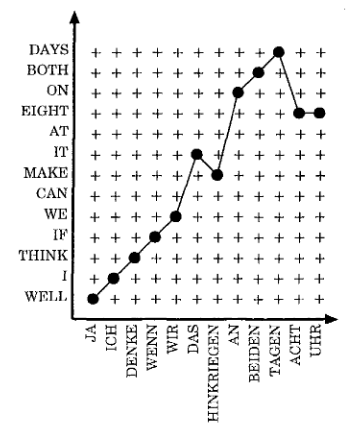
\includegraphics[scale=0.4]{figures/alignment.png}
        \vspace*{-2mm}
    \end{center}
    \caption{Word alignment for a German-English sentence pair~\cite[Figure 1]{vogel1996hmm}.}
    \label{fig:alignment}
\end{figure}

\subsection{Natural language understanding}
\label{subsec:nlu}
Conversational agent or dialogue systems aim to communicate with humans using natural language.
Consensus is not clear on whether a chatbot is synonymous to conversational agent.
Some argue it is~\citep{io2017chatbots}, and some argue that conversational agents are more sophisticated that bots which can chat.
This thesis will consider the words to be synonymous.
Conversational agents can be used to replace graphical user interfaces~\citep{brennan1990conversation} or to act as a social companion~\citep{fitzpatrick2017delivering, zhou2018design}.
Interpreting user utterances gives rise to a new tasks, often denoted as natural language understanding (NLU)~\citep{jaech2016domain, braun2017, yang2017end}.
NLU extracts information from user sentences.
The meaning for the entire sentence or intention is defined as an intent.
Information from one or more sequential words is defined as a named-entity.
For example consider the following sentence:

\begin{center}
"I would like to book a ticket to London tomorrow."
\end{center}

In this sentence the intent of the user is to book a ticket.
Conversational agents which handle these requests have some related slots which need to be filled.
For this book ticket example the system needs to know the destination of the user and when the user wants to arrive.
Named-entity recognition (NER) can be used to find this information.
A NER classifier can be trained to classify London as a destination and tomorrow as a date.
Most systems allow entities to be defined by examples and regular expressions.
The examples can be used for keyword matching or entities similar to the examples can be detected by using machine learning.

\section{Deep learning}
\label{sec:deep_learning}

As with many computer science subfields deep learning has outperformed manual feature engineering on many NLP tasks.
For the last few years the best performing NLP systems have been neural networks.
This section will provide a basic overview of the most important model architectures.
% TODO: Explain encoder decoder.
% TODO: Explain transfer learning? (used for ELMo)

\iffalse
\subsection{word2vec}
\label{subsec:word2vec}
This section will take one step in the direction of using deep learning for NLP.
Neural networks are basically a mapping from vector to vector (numbers to numbers).
Natural language can be converted from and to vectors using embeddings.
This section will introduce embeddings and explain some common concepts.
The focus lies on the intuition behind the approaches.
The goal of this is being able to estimate suitability of certain approaches for certain tasks.


\subsection{GloVe}
\label{subsec:glove}
\fi

\subsection{Vanishing gradient problem}
\label{subsec:vanishing_gradient_problem}
The vanishing gradient problem has for a long time halted the progress of neural networks with many layers, also known as deep neural networks.
Backpropagation updates the weights in the network by sending information from the output layer in the direction of the input layer.
The problem relates to vanishing and exploding updates to weights in the layers further from the output layer.
These extreme updates are caused by the backpropagation algorithm.
Consider some weight $w$ which is near the input layer of some network.
Say this weight is updated by the following partial derivative $w = d_1 \cdot d_2 \cdot \ldots \cdot d_i$.
Here $i$ denotes the number of layers in the network.
These partial derivatives $d_x$ can become small $(0 \leq d_x < 1)$ or large $(1 \ll d_x)$.
Typically the learning rate has an order of magnitude of \num{1e-3}.
When one derivative is small the weight update when multiplied by learning rate might become very small.
Conversely when one derivative is big the update might become very big.
Since the weight is near the input layer $i$ is big.
Thus, the chance that weights further away from the output layer vanish or explode increase by increment of $i$.
Effectively the problem causes layers which are have a long distance from the output layer to stop learning.

\subsection{Recurrent neural networks}
\label{subsec:rnn}
\begin{figure}[htbp]
    \begin{center}
        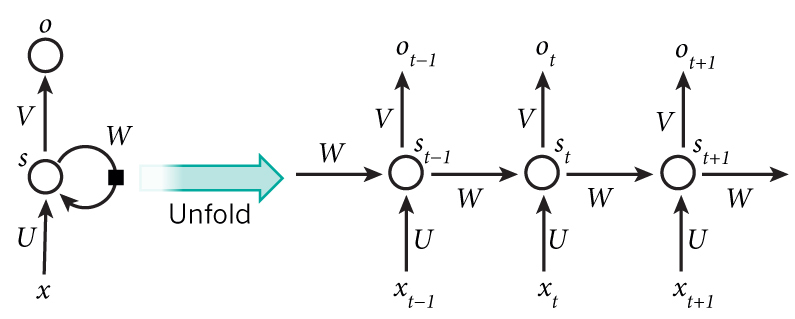
\includegraphics[width=0.5\textwidth]{figures/rnn.jpg}
    \end{center}
    \caption{Recurrent neural network~\cite[Figure 5]{lecun2015deep}.}
    \label{fig:rnn}
\end{figure}
A recurrent neural network (RNN) is an extension on neural networks which allows the network to have memory.
Simply put the network remembers a summary of information from all previous states.
A common way to visualize this is depicted in figure~\ref{fig:rnn}.
On the right side the model is unfolded in time.
The unfolded representation shows the state of the network and the flow of information for three consecutive points in time.
To access this history the neural network in current state $s_t$ obtains a `summary' from the previous state $s_{t-1}$.
Suppose we are training a RNN in an unsupervised way.
The model trains on real-world texts.
For each word $w_i$ it is asked to predict $w_i$ based only on previous words $w_1, w_2, \ldots, w_{i-1}$.
In the image $w_i$ is denoted as input $x_i$.
After predicting the prediction is compared to the correct word, if these are not equal the loss is backpropagated.
The backpropagation is then able to `change history' to improve prediction accuracy.

The benefit of this architecture over n-grams is that the information is compressed inside the neural network.
Also, there is a certain sense of importance since the weights are not uniformly updated for all previous states (words).
Take, for example, `the car, which is green, broke'.
For this sentence the word `broke' can more easily be predicted based on `the car' than on `which is green'.

In practice RNNs are not using the complete history.
The cause for this are vanishing and exploding gradients.
Large updates can be detected and solved by putting a threshold on the updates~\citep{mikolov2014learning}.
Small updates however can either be caused by vanishing gradients or by the fact that the weight should not be updated.
In practise gradients vanish and simple RNNs become like 7-grams for most words~\citep{manning2017lectures}.

\subsection{Gated recurrent units and LSTMs}
\label{subsec:gru}
Basic RNNs do not yet provide a way to translate languages.
Machine translation requires to convert some sentence from a source language to a target language.
To this end a RNN encoder-decoder has been proposed by~\citet{cho2014learning}.

\begin{figure}[htbp]
    \begin{center}
        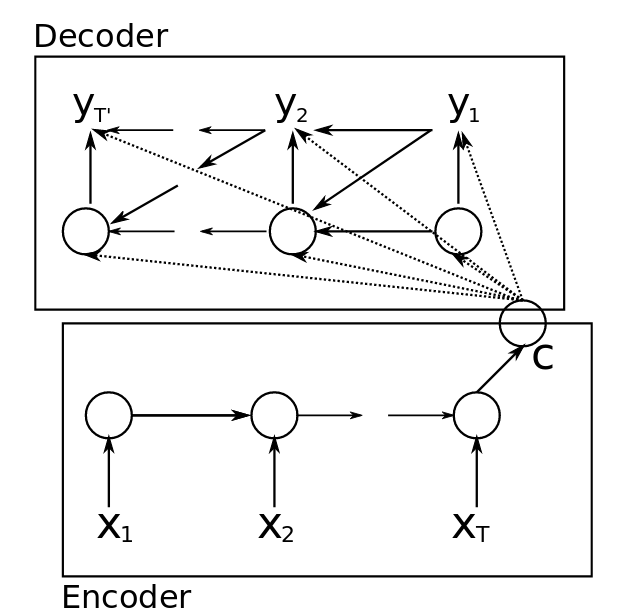
\includegraphics[width=0.5\textwidth]{figures/encoder_decoder.png}
    \end{center}
    \caption{RNN Encoder-decoder~\cite[Figure 1]{cho2014learning}.}
    \label{fig:encoder_decoder}
\end{figure}

Similar to the basic RNN the decoder at some time has access to only the previous state, see figure~\ref{fig:encoder_decoder}.
The encoder takes the source sentence of variable length $T$ and maps it to a fixed length vector.
The decoder in turn maps the fixed length vector to the target sentence of length $T'$.
To do this the network reads all words $x_1, x_2, \ldots, x_T$ until an end of line token is received.
At that point the entire sentence is captured in the hidden state $C$.
The decoder starts generating words $y_1, y_2, \ldots, y_{T'}$ based on the previous decoder states and $C$.
This is visualised by the arrows.
The authors of the paper recognized that this approach has the same limitations as the basic RNN.
Typically words in translation sentence pairs are somewhat aligned, as described in subsection~\ref{subsec:mt}.
For example, when generating the first word $y_1$ the algorithm mainly needs info from $x_1$, but has more recently seen the next words in the sequence $x_2, x_3, \cdots, x_{T'}$.
Vanishing gradients will cause the network to forget its far history, so this methods does not work well for long sentences.
To solve this the authors have also introduced gates to RNNs.

\begin{figure}[htbp]
    \begin{center}
        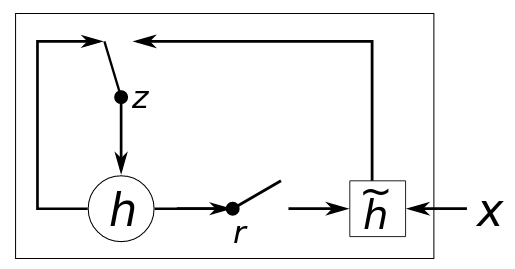
\includegraphics[width=0.5\textwidth]{figures/gru.png}
    \end{center}
    \caption{GRU hidden activation function~\cite[Figure 2]{cho2014learning}.}
    \label{fig:gru}
\end{figure}

Gated recurrent units (GRUs) have gates which automatically learn to open and close for some hidden state.
This can be visualised by looking at the information which is passed through the states.
The information is captured in a matrix.
In a RNN the information in the entire matrix is updated in each step.
GRUs learn to read and write more selectively, see figure~\ref{fig:gru_subset}.
For some point in time the update consist of reading a specific subset and writing a specific subset of the matrix.
In effect the network learns to look only at the word it needs~\citep{manning2017lectures}.
For example when translating a sentence from German to English it will look at the verb in German to come up with the verb in English.
Writing, in effect, lets the model allocate specific parts in the matrix for specific parts of speech (for example, nouns and verbs).

\begin{figure}[htbp]
    \begin{center}
        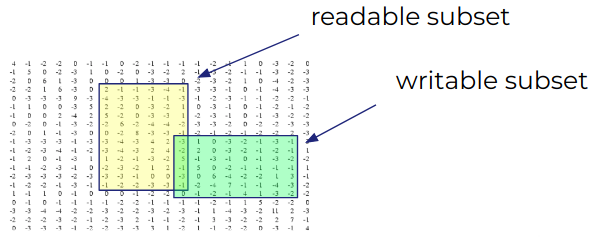
\includegraphics[width=0.5\textwidth]{figures/gru_subset.png}
    \end{center}
    \caption{Simplistic visualisation for updating the hidden state in a GRU.}
    \label{fig:gru_subset}
\end{figure}

Long short-term memory networks (LSTMs)~\citep{hochreiter1997long} are similar to GRUs.
An LSTM does not only contain update and reset gates but also uses a internal memory state.
In practise LSTMs take longer to converge than GRUs~\citep{chung2014empirical}, but remember around 100 words where GRUs remember around 40.

\iffalse
\subsection{Attention}
\label{subsec:attention}
%See also CS224n including 'advanced attention' slides.
One drawback of recurrent neural networks using the encoder-decoder model is that the decoder obtains all information from the final state of the encoder.
A problem with this can be explained by looking at machine translation.
When translating words are aligned as explained in section~\ref{subsec:mt}
When generating the $n$-th word during decoding information we generally need mainly information from the $n$-th word which occurred during encoding.
It makes more sense to focus the neural network \textit{attention} on the part of the sentence we actually need the most.
To this end the neural net learns to choose what hidden states are important.
%TODO: Really add image here just like slides.
% The important states get a higher weight which yield a context vector.
% TODO: Way too short, need to explain better.
\fi

\subsection{Bidirectional recurrent neural networks}
\label{subsec:bidirectional}
All recurrent architectures described above use only the information on the left of some word to predict it.
Take for example the following sentences containing the polyseme `drinking'.
\begin{center}
    Peter was drinking after a workout.\\[3mm]
    Peter was drinking excessively.
\end{center}
The meaning of the word `drinking' changes after reading the next words in the sentence.
To take this into account bidirectional recurrent neural networks (BRNN) have been developed by~\citet{schuster1997}.
A BRNN contains two separate RNNs as depicted in figure~\ref{fig:bidirectional}.
The paper only considers RNNs, but the method can be applied to gated recurrent models as well.
One RNN goes through elements of the sequence from left to right and the other in the reverse direction.
Training can be done by showing the network all words except for one.
Both networks learn to predict the next word given a sequence of words.
Calculating the loss is done by taking the average of the predictions of both RNNs.
To reduce required computational power one simplification is used.
Suppose we want to learn from the word at location $k$, $w_k$.
A solution would be to get all the way to states $s_{k-1}$ and $s_{k+1}'$ to predict $w_k$.
Then we update the weights and, assuming we go forward, now want to learn from $w_{k+1}$.
The RNN in state $s_{k-1}$ takes one step forward, but the RNN in state $s_{k+1}'$ has to restart from the last word in the sequence.
To solve this both RNNs make one prediction for each word and the answers of both for the entire sequence are used to update the weights.

\begin{figure}[htbp]
    \begin{center}
        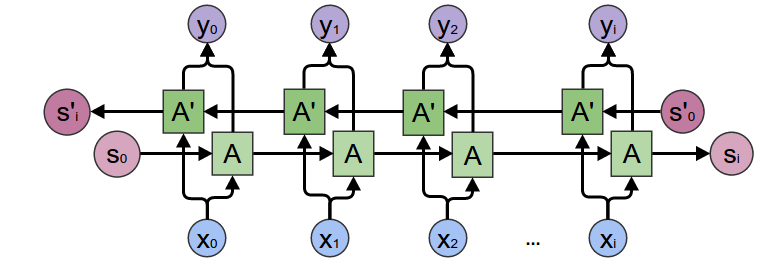
\includegraphics[width=0.5\textwidth]{figures/bidirectional.png}
    \end{center}
    \caption{Bidirectional RNN~\citep{olah2015}.}
    \label{fig:bidirectional}
\end{figure}

\subsection{Convolutional neural networks}
\label{subsec:cnn}
% cnn intro
Convolutional neural networks (CNNs) are an extension to vanilla neural networks which allow the model to exploit spatial locality.
This makes the networks highly successful for image classification.
During image classification CNNs learn a hierarchical representation of the input, according to~\citet{conneau2016very}.
The authors claim that such an hierarchical representation would have benefits for NLP over sequential models.
One of the benefits is that the depth of the tokens, which can be chosen as words but also characters, varies for the tokens in the sentence.
In CNNs this depth would be constant, which mitigates the problem of forgetting tokens seen in a less recent past.

% cnn outro
A review by~\citet{young2018recent} argues that CNNs are suited for specific NLP tasks.
When data is scarce they are not effective.
Foundational problems with CNNs are that they are unable to model long-distance contextual information and preserving sequential order.
The former implies that CNNs are not well suited for question answering tasks.

\subsection{ELMo}
\label{subsec:elmo}
Word embeddings generated by competitive models such as Word2vec~\citep{mikolov2013distributed} and GloVe~\citep{pennington2014} do not take context into account when determining word representations.
For ELMo ``each token is assigned a representation that is a function of the entire input sentence''~\citep{peters2018}.
This is done by using a bidirectional LSTM.
To improve accuracy further the authors advise to use the deep internals of the network.
These internals can be used for downstream models.
For example, the authors show that word sense disambiguation tasks are captured by higher level LSTM states.
Part-of-speech tagging or named entity recognition are captured by lower level states.
ELMo is not the first system to use context, but was obtaining state-of-the-art empirical results on multiple non-trivial tasks at the time of publication.
Another reason for this is that the system is character based.
Word based systems cannot generate an embedding for a word they have not seen during training (out-of-vocabulary tokens).
In character based systems morphological clues can be used to guess the meaning of the out-of-vocabulary words.
The system has quickly become very popular.
Reasons for this seem to be that the system generalizes well, and is trained on a lot of data.
The model is integrated into the AllenNLP open-source NLP library created by~\citet{gardner2017}.

\subsection{Transformers}
\label{subsec:transformers}
The main issue in the recurrent approaches is that distant information needs to pass through all the intermediate states.
In the basic RNN for each state all the information is updated, causing less recent information to gradually disappear.
Gated recurrent architectures (GRUs and LSTMs) reduce this problem by being more selective when viewing or changing information.
Transformer networks allow the model to look at previous inputs instead of previous states~\citet{vaswani2017attention}.
For example, suppose we are translating `impounded' in the following sentence pair from the WMT'14 English-German dataset.
\begin{center}
    The motorcycle was seized and \underline{impounded} for three months.\\[3mm]
    Das Motorrad wurde sichergestellt und f\"ur drei Monate \underline{beschlagnahmt}.
\end{center}
Suppose the system has correctly predicted the German sentence up to and including `Monate'.
The next step is to predict `beschlagnahmt'.
To do this the system needs mainly information about the word `impounded'.
Gated recurrent architectures learn to look at the previous state in such a way that the attention is focused on `impounded'.
This requires the information of the word to not been overwritten during execution.

Transformers evade this overwriting problem by allowing the system to see all $d$ previous words, where $d$ is 1024 for the biggest model.
The only thing the transformer then needs to learn is where to focus its attention.
The information of all the previous words is stored in an array of word vectors (a tensor).
To apply focus to parts of this tensor the model learns to put a mask over the tensor.
In the mask zeroes correspond to hidden items.
One drawback is the required computational power.
Suppose we only need one word from the $d$ previous words.
The mask will hide $d-1$ words.
This still requires to multiply the masked word vectors by infinity.
Google argues that this is not really an issue since matrix multiplication code is highly optimized and graphic processing units (GPUs) and tensor processing units (TPUs) exist.
So, the model can relate any dependency in constant time when the range is lower than $d$.
This in contrast to recurrent layers which are in linear time.
When the sequence length is greater than $d$ computations will require more than linear time.

Another benefit of the transformers are that self-attention visualisations can more easily be done than in recurrent architectures.
By self-attention the authors refer to attention that is used to generate context aware word representations.
An example of a tranformer model correctly applying coreference resolution is presented shown in figure~\ref{fig:coreference_resolution}.

\begin{figure}[htbp]
    \begin{center}
        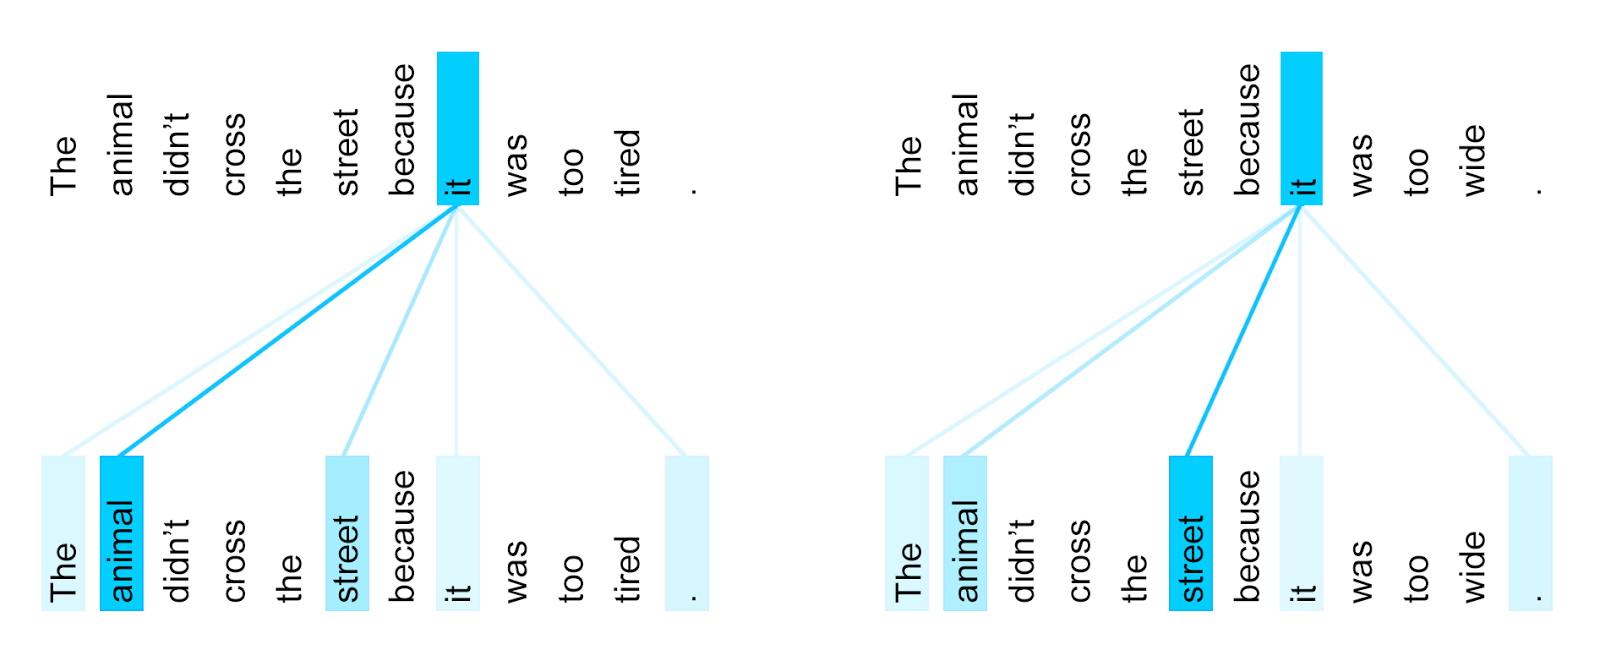
\includegraphics[width=\textwidth]{figures/coreference_resolution.png}
    \end{center}
    \caption{Encoder self-attention distribution~\citep{uszkoreit2017}.}
    \label{fig:coreference_resolution}
\end{figure}

\iffalse
\subsection{BERT}
\label{subsec:bert}
WordPiece tokenization, as published by~\citet{wu2016}, is used.
They argue that the tokenization ``provides a good balance between the flexibility of `character'-delimited models and the efficiency of `word'-delimited models''.
\fi


    \clearemptydoublepage

    \chapter{Benchmarking}
\label{ch:benchmarking}

This chapter aims to answer the first research question.
The goal is to create a reproducible benchmark tool, simply called \textsc{bench}.
Datasets used by the benchmark tool are described in section~\ref{sec:datasets}.
The benchmarked systems are described in section~\ref{sec:systems}.
Running the benchmarks on various datasets and systems resulted in scores, see section~\ref{sec:benchmark_results}.
It has been found that \textsc{bench} is impractical, described in section~\ref{sec:issues}.
Notes on using the tool and a high-level overview is presented in appendix~\ref{ch:bench}.

\section{Datasets}
\label{sec:datasets}
Trained models are considered black boxes at the time of writing.
To verify performance of a model data is required.
This is fed to the model and results are measured.
This section will describe the datasets used for benchmarking.

\subsection{Format}
\label{subsec:format}
The dataset format needs to be able to specify a sentence annotation and subsentence annotation.
% NER only annotations
One often used dataset for subsentence, or token, classification is CoNLL-2003~\citep{tjong2003}.
It uses the NER task definition as described by~\citet{chinchor1999}.
The definition uses tags to specify entities, for example:
\begin{center}
    \begin{verbatim}
        <B_ENAMEX TYPE="PERSON">bill<E_ENAMEX> and <B_ENAMEX TYPE="PERSON">
        susan jones<E_ENAMEX>
    \end{verbatim}
\end{center}
Note that this constraints the text since angled brackets (`$<$', `$>$') cannot be used without escaping the brackets.
A less verbose and non text constraining annotation standard is the BIO2 annotation standard.
The origin is unclear, but adaptation is done by at least Stanford as seen in the GloVe paper~\citep{pennington2014}.
Here sentences are annotated as follows.
\begin{center}
    \begin{verbatim}
        I B-Person
        and O
        John B-Person
        Doe I-Person
        worked O
        yesterday B-Date
        . O
    \end{verbatim}
\end{center}
where B, I and O respectively mean begin, intermediate and `empty' annotation.
Note that other annotations, like part-of-speech tagging, are possible by adding another column of tokens.
A benefit of this annotation is that measuring performance can be done by looking at each token annotation separately.
In a tag example like above it is unclear how cases where the classifier is partly correct should be solved.
Suppose only `susan' is classified as person and not her last name `jones'.
Metrics now have to decide how to handle this partially correct situation.
In the BIO2 annotation standard token classifications can only be correct or incorrect.
One drawback is that the standard is not easy to read for humans.
A more readable format is the Rasa Markdown format.
Here it constraints the text by using square (`[', `]') and round bracket (`(', `)') symbols to denote annotations.
For example:
\begin{center}
    \begin{verbatim}
    [I](person) and [John Doe](person) worked [yesterday](date).
    \end{verbatim}
\end{center}
Unlike BIO2 this standard does not easily allow to also specify other annotations, for example part of speech tagging.
One could argue that the readability of a Markdown format and the versatility of the BIO standard show that there is no single best approach.

% combined annotations
A combination of sentence annotations and token annotations is not supported by the standards described above.
For BIO one could track the sentence annotations in a separate file or put it before or after the sentence.
The former adds duplicate information while the latter makes the file incompatible with the standard.
For Rasa one could change it to a tab separated file and put the Markdown and sentence annotation in separate columns.
This is very readable and compact, but means transforming the multi-token annotations to separate token annotations for easier validation.
Datasets which combine sentence annotations with token annotations seem to take yet another approach.
They use json to store any information they have.
These formats should allow for easier parsing, but can not easily be read by humans.
For example one dataset annotates entities as as follows.
\begin{center}
    \begin{verbatim}
        "entities": [{
        "entity": "StationDest",
        "start": 4,
        "stop": 4,
        "text": "marienplatz"
        }]
    \end{verbatim}
\end{center}
This entity belongs to the sentence ``i want to go marienplatz''.
`start' and `stop' here assume the sentence to be tokenized using a WordPunctTokenizer~\citep{bird2004nltk} having regexp \verb/\w+|[^\w\s]+/.
Drawbacks are that the entity text is duplicated and that the datasets are hard to read for humans.
The sentences have to be manually tokenized for verification and the number of lines of the dataset is an order of magnitude higher than the Markdown format.

\subsection{Available datasets}
\label{subsec:available_datasets}
% nlu evaluation corpora
Three datasets for intent classification and entity recognition are created and made publicly available by~\citet{braun2017}.
The paper and its Github version use different names, this thesis will stick to WebApplications, AskUbuntu and Chatbot.
WebApplications and AskUbuntu are obtained by pulling questions from StackExchange\footnote{\url{https://stackexchange.com}}.
For example, they respectively contain ``How can I delete my [Hunch](WebService) account?'' and ``How to install a [Brother MFC-5890CN](Printer) network printer?''.
Intents for these examples are respectively `Delete Account' and `Setup Printer'.
StackExchange datasets are labeled using Amazon Mechanical Turk.
The Chatbot dataset is based on a Telegram chatbot in production use.
This dataset contains sentences like ``when is the [next](Criterion) [train](Vehicle) in [muncher freiheit](StationStart)?'' having intent `DepartureTime'.
Labeling for Chatbot is done by the authors of the paper.

% snips
Snips~\citep{snips2019voice} is a company which provides software to locally run a voice assistant.
They have shared some of the data generated by their users as well as results for their benchmarks~\citep{snips2017dataset}.
The incentive for sharing these datasets seems to be showing that their system performs better than other systems.
Two datasets have been published by Snips.
The thesis has only used the 2017 version and not the 2016 version.
The 2017 version will from now on be referred to as Snips2017.
Sentences in this dataset are typically short.
They utter some command to the system, for example for the intent `PlayMusic': ``i want to listen to [Say It Again](track) by [Blackstratblues](artist)''.

% table description and general info
Full datasets can be inspected at Github\footnote{\url{https://github.com/rikhuijzer/nlu\_datasets}}.
Summary statistics for these datasets are listed in Table~\ref{tab:corpora}.
In this table `None' is not counted as an intent.
The reason for specifying this is that falling back to \textit{null} or some intent during unsure predictions result in different scores for most metrics.
$\text{F}_1$ score calculations, for example, do not ignore \textit{nulls} or `None', but instead consider them as a separate group.
Information about the unique number of entities for Snips2017 is not specified by the dataset authors.

% summaries of data
\begin{table}
    \centering
    \begin{tabular}{l l l l l}
        \textbf{Dataset} & \textbf{Train} & \textbf{Test} & \textbf{Intents} & \textbf{Entities}\\
        \hline
        WebApplications & 30 & 54 & 7 & 1\\
        AskUbuntu & 53 & 109 & 4 & 3\\
        Chatbot & 100 & 106 & 2 & 5\\
        Snips2017 & 2100 & 700 & 7 & unknown\\
    \end{tabular}
    \caption{Number of labeled train and test sentences and unique intents and entities per dataset}
    \label{tab:corpora}
\end{table}


\section{Systems}
\label{sec:systems}

\subsection{Rasa}
\label{subsec:rasa}
% introduction
Rasa (\url{https://rasa.com/}) is an open-source system allowing users to build conversational agents.
The systems consists of two parts, namely \textsc{rasa\_nlu} and \textsc{rasa\_core}.
The former classifies sentences and sub-sentences.
To train the system users can specify (hierarchical) intents, synonyms and regexes.
Hierarchical intents is a recent addition which allows the system to extract multiple intents from a sentence.
For example, it can extract `hi+book\_ticket' from
``Good morning.
Can I order a ticket to London please?''.
The system is actively used in production.
As a result the code is well documented and stable.

% dialogue management
\textsc{rasa\_core} aims to handle dialogue management.
This is an extension on the classifiers of \textsc{rasa\_nlu} which aims to understand text in context.
Also, it can be used to specify conversation flow.
This part remains one of the most difficult problems for conversational agents.
Humans tend to switch rapidly between topics in conversations.
For example, suppose one ticket order conversation flow contains six questions to be answered by the customer.
Customers expect to be able to switch topic during each one of these questions and then return to the flow.
Enabling this behaviour via state machines or flowcharts is cumbersome, because the number of transitions tends to grow quickly.
One of the Rasa solutions is applying machine learning to let developers train dialog flows interactively.

% using system
Rasa allows the system to be used as API and `Python API'.
The Python API is the most efficient.
Here users install \textsc{rasa\_nlu} in their programming environment and call functions directly.
Depending on the used back-end a selection of dependencies have to be installed.
Since Rasa is called from Python it is not able to maintain a state.
The regular API advises to spin up a Docker container.
This is less efficient, but more modular.
Containers are published to Docker Hub by Rasa.
Users can pull these for free and use the newest stable configuration of choice.

% back-ends or pipelines
Configurations are defined as a pipeline.
Pipelines specify what components should be applied to sentences and in what order.
Typical pipelines contain at least a tokenizer followed by some classifier.
Pipelines are meant to be modified easily and specified in yaml.
In practise default pipelines often suffice for end-users.
A back-end refers to the used intent classifier in some pipeline, for example `tensorflow'.
At the time of writing three back-ends are offered by Rasa, namely \textsc{rasa-mitie}, \textsc{rasa-spacy} and \textsc{rasa-tensorflow}.
\textsc{rasa-mitie} is the oldest and depreciated.
Training MITIE (\url{https://github.com/mit-nlp/MITIE}) takes at least a few minutes for small datasets.
This is caused by the fact that it is tuning hyperparameters during training.
On two computers used for this thesis the Docker Hub image occasionally hangs on various datasets.
\textsc{rasa-spacy} is the successor of MITIE and, unsurprisingly, based on spaCy (\url{https://spacy.io}).
In 2015 spaCy was in the top 1\% for accuracy and the fastest syntactic parser~\citep{choi2015depends}.
spaCy (and by that \textsc{rasa-spacy}) requires a language model to parse text.
It includes seven language models for which English, Spanish and French include vectors.
The multilingual model supports only named entities.
Unlike the other two back-ends \textsc{rasa-tensorflow} is not based on a pre-trained language model.
This is like classifying sentences in an unfamiliar language (say Chinese) after only seeing some examples.
Rasa advises to use this back-end when training data contains more than 1000 training examples.
The benefit is that this back-end is language independent and can handle domain specific data and hierarchical intents.

\subsection{DeepPavlov}
\label{subsec:deeppavlov}
DeepPavlov~\citep{burtsev2018} is similar to Rasa.
Unlike Rasa, DeepPavlov aims to aid researchers in development of new techniques for conversational agents.
Being a newer system than Rasa and aimed at researchers the system is not yet production ready.
The system does only provide a Python API, requiring Python 3.6.
One claimed benefit of the system is that they do not export machine learning components from other systems.
Another reason why the system is not well suited for production is that pipelines can download information.
This means that a generic Docker needs to download many megabytes of data for each time the Docker is started.
Manually defining new Dockers holding this information is possible, but does require some knowledge about Docker and some time to set it up.
For users who want to use few training examples pre-trained models are necessary.
DeepPavlov by default includes DSTC 2, Wikipedia, Reddit, RuWiki+Lenta and ELMo embeddings.
Its hard to tell what model should be chosen for some use-case.

% cloud services
\subsection{Cloud services}
\label{subsec:cloud_services}
% conversational agents
Cloud service providers and various small companies (start-ups) provide APIs for conversational agents.
Functionality differs per provider, but in the basis they all over the same features.
Naming conventions do not seem to exists.
For example, Rasa calls intent classification training examples \textit{utterances}, while Google Dialogflow calls them \textit{training phrases}.
Via the web interface or API examples can be sent to a server and the system can be configured.
Configurations specify the utterances, dialog flows, how to classify entities (used for slot filling) and input language.
At some point the server will use the provided examples to train the model.
This takes a few seconds.
This makes sense, since users do not want to wait and computations cost money.
Settings for the dialogs and APIs are located somewhere in the complete cloud offerings.
An extension on the intent classification and slot filling described above is using knowledge bases.
When looking at IBM Watson a document needs to be uploaded and annotated by humans.
This is an example of a structured knowledge base.

% list of further natural language understanding providers
In the period that IBM Watson won the Jeopardy quiz a lot of math and reasoning was required to create NLP systems.
Nowadays, training a competitive neural network for natural language processing is relatively easy.
It takes a PhD candidate a few months~\citep{manning2017lectures}.
This results in a lot of companies providing natural language processing services.
An in-depth analysis of all services is left out.
The following is a non-exhaustive list.
Some offer full conversational agent capabilities, while others focus on natural language understanding.
\begin{description}
    \item [Watson Assistant (\url{https://www.ibm.com})] is a conversational agent by IBM.
    \item [Dialogflow (\url{https://dialogflow.com})] is a conversational agent by Google.
    \item [Lex (\url{https://aws.amazon.com/lex})] is a variant created by Amazon.
    \item [wit.ai (\url{https://wit.ai})] can be used for chatbots and is acquired by Facebook.
    The system is free to use, but Wit is allowed to use the data sent to their servers.
    \item [Deep Text (\url{https://deeptext.ir})] provides sentiment analysis, text classification, named-entity recognition and more.
    \item [Lexalytics (\url{https://www.lexalytics.com})] provides categorization, named entity recognition, sentiment analysis and more.
    \item [Pat (\url{https://pat.ai})] has as goal to humanize AI and provides some conversational agent services.
    \item [kore.ai (\url{https://kore.ai})] focus lies on intent classification and entity extraction with as goal to replace graphical user interfaces with chatbots.
\end{description}
Sixteen more are listed by~\citet{dale2018text}.


\section{Tool and results}
\label{sec:bench}
% intro
The benchmarking tool is called \textsc{bench} and available on Github\footnote{\url{https://github.com/rikhuijzer/bench}}.
Its goal is to be a reproducible benchmarking tool for intent classification and named-entity recognition.
Reproducible means that anyone can clone and run the code to reproduce the results presented in this thesis.
The code is written in Python, since it is the default choice for machine learning.
Python is conceived as a object-oriented language.
Over time it has included more and more functional programming ideas.
The code in this project will aim to be adhering to functional programming.
Reasons are pedagogic value, improved modularity, expressiveness, ease of testing, and brevity.
Some general notes on functional programming in Python are listed in Appendix~\ref{ch:fp}.

% final code remarks on fp and imports
The functional programming constraints for the project are that we do not define any new classes.
Specifically, we do not use the class keyword.
Exceptions being NamedTuples and Enums.
The code prefers returning iterators over collections, the reason for this is explained in Appendix~\ref{ch:demonstration}.
A final remark is about the imports.
When importing, an attempt is made to explicitly import using `from $<$module$>$ import $<$class$>$'.
When more implicit imports are used `import $<$module$>$' this is can have multiple causes.
It is either caused by the appearance of circular imports, by the fact that some names are too common or to avoid reader confusion.
An example for the latter are the types defined in \textsc{src.typ}.
The names are quite generic and could cause name clashing or confusion when imported explicitly.

\subsection{Overview}
\label{subsec:overview}
Since the code does not contain classes, the high-level overview is simply a tree-like structure.
This is analogous with a book, where subsections are contained in sections and sections are contained in chapters.
In the code small functions are called by larger functions and these larger functions are called by even larger functions.
For an overview this idea can be generalized to modules.
An overview for the modules of \textsc{bench} is roughly as follows.
The `.py' suffix is omitted for all elements in the tree.
Tests are also omitted.

\begin{itemize}
    \item \textsc{bench}
    \begin{itemize}
        \item \textsc{src.utils}
        \item \textsc{src.typ}
        \item \textsc{src.dataset}
        \begin{itemize}
            \item \textsc{src.datasets.corpora}
            \item \textsc{src.datasets.snips}
        \end{itemize}
        \item \textsc{src.system}
        \begin{itemize}
            \item \textsc{src.systems.amazon\_lex}
            \item \textsc{src.systems.deeppavlov}
            \item \textsc{src.systems.dialogflow}
            \item \textsc{src.systems.mock}
            \item \textsc{src.systems.rasa}
            \item \textsc{src.systems.watson}
        \end{itemize}
        \item \textsc{src.evaluate}
        \begin{itemize}
            \item \textsc{src.results}
        \end{itemize}
    \end{itemize}
\end{itemize}

Some generic functions are listed in \textsc{src.utils} and used through the entire project.
The project makes use of type hints as introduced in Python 2.7.
All NamedTuples or `types' are defined in \textsc{src.typ}.
An overview of the most important types is depicted in Figure~\ref{fig:types}.
These types also contains enumerables or `Enums'.
These are used in cases where function behaviour depends on some parameter having a fixed set of options.
Alternatively one could use strings for these cases depending on user-preference.
Notable is the usage of \textsc{System}, and by that the usage of \textsc{Corpus}, in \textsc{Query}, \textsc{SystemCorpus}, \textsc{Classification} and \textsc{F1Score}.
This is caused by the fact that external systems (for example, DialogFlow) have a certain state which needs to be passed through many functions.
This state could be that the system has not yet seen the dataset, resulting in \textsc{Corpus.EMPTY}, or the system has trained on AskUbuntu, which results in \textsc{Corpus.ASKUBUNTU}.
In, for example, \textsc{Classification} this is used to let some evaluation function know context for an input sentence.
This context includes from what dataset the sentence came and what system has classified the sentence.

% Define block styles
\tikzstyle{block} = [rectangle, draw, fill=blue!20,
    text width=6em, text centered, rounded corners, minimum height=4em]
\tikzstyle{line} = [draw, -latex']
\tikzstyle{cloud} = [draw, ellipse,fill=red!20, node distance=3cm, minimum height=2em]
\tikzstyle{small_block} = [rectangle, draw, fill=blue!20,
    text width=5em, text centered, rounded corners, minimum height=4em]

\begin{figure}[htbp]
    \centering
    \begin{tikzpicture}[node distance = 3cm, auto]
        % Place nodes
        \node [small_block] (0) {System};
        \node [small_block, left of=0] (10) {Corpus};
        \node [small_block, below of=0] (1) {System-\\Corpus};
        \node [small_block, left of=1] (2) {Query};
        \node [small_block, right of=0] (3) {Response};
        \node [small_block, right of=1] (4) {Classi-\\fication};
        \node [small_block, right of=4] (5) {F1Score};

        \node [small_block, below of=1] (6) {CSVStats};
        \node [small_block, left of=6] (7) {CSVIntent};
        \node [small_block, right of=6] (8) {CSVEntity};
        \node [small_block, right of=8] (9) {CSV};

        \path [line] (10) -- (0);
        \path [line] (0) -- (1);
        \path [line] (10) -- (1);
        \path [line] (0) -- (2);
        % to classification
        \path [line] (0) -- (4);
        \path [line] (3) -- (4);
        % to f1 score
        \path [line] (0) -- (5);
    \end{tikzpicture}
    \caption{Overview of most important type classes (NamedTuples and Enums) and their relations in \textsc{bench}.
    Here a line from $A$ to $B$ means that $B$ is a type which includes $A$ ($B$ extends $A$).}
    \label{fig:types}
\end{figure}

The real work of the project is done by \textsc{src.dataset}, \textsc{src.system} and \textsc{src.evaluate}, as shown in Figure~\ref{fig:flowchart}.
`Dataset' takes input files and converts them to an internal representation as defined by \textsc{src.typ}.
Input files here denote the original dataset files as created by the dataset publishers.
For the internal representation a Rasa Message\footnote{\textsc{rasa\_nlu.training\_data.message.Message}} is used.
The benefit of this is that it avoids defining the same structure and that it can be used in combination with Rasa code.
For example, \textsc{src.dataset.convert\_message\_to\_annotated\_str} uses Rasa code to print the internal data representation as a sentence in Markdown format (Section~\ref{subsec:format}).
Next, the data reaches \textsc{src.system}.
Here it is passed to the system under consideration, either in training or prediction mode.
For the predictions this is done by finding out which function can convert \textsc{src.typ.Query} to \textsc{src.typ.Response}.
When, for example, Rasa is under consideration the function \textsc{src.systems.rasa.get\_response} is called.
DeepPavlov would be handled by \textsc{src.systems.deeppavlov.get\_response}.
PyCharm is known to have the best type inference for Python.
The IDE is not yet able to infer function type for a function mapping, even when all functions have the same input and output type.
A workaround is to manually define the type of the function returned by the mapping as \verb|func: Callable[[tp.Query], tp.Response] =| $\cdots$.
\textsc{src.evaluate} takes all responses \textsc{tp.Response} evaluates the performance of the system under consideration.
Printing $\text{F}_1$ score is a matter of three functions and about a dozen lines of code.
At one point more advanced logging has been included which is responsible for the other 12 functions and 110 lines of code.

\begin{figure}[htbp]
    \centering
    \begin{tikzpicture}[node distance = 2cm, auto]
        % Place nodes
        \node [block] (srcdataset) {\textsc{src.dataset}};
        \node [cloud, above of=srcdataset] (dataset) {dataset};
        \node [block, below of=srcdataset] (srcsystem) {\textsc{src.system}};
        \node [cloud, right of=srcsystem] (system) {system};
        \node [block, below of=srcsystem] (srcevaluate) {\textsc{src.\\evaluate}};
        \node [cloud, below of=srcevaluate] (score) {\fone score};
        % Draw edges
        \path [line] (dataset) -- (srcdataset);
        \path [line] (srcdataset) -- (srcsystem);
        \path [line] (srcsystem) -- (srcevaluate);
        \path [line] (srcevaluate) -- (score);
        \path [line] (srcsystem) -- (system);
        \path [line] (system) -- (srcsystem);
    \end{tikzpicture}
    \caption{Diagram showing the dataflow in \textsc{bench}.}
    \label{fig:flowchart}
\end{figure}

\subsection{Benchmark results}
\label{subsec:benchmark_results}
This section presents the benchmark results for intent classification using \fone scoring with micro averaging.
\fone formulas are listed in Section~\ref{subsec:f1_score}.
An explanation for the differences in averages for the \fone score is presented in Section~\ref{subsec:methodology}.
Here micro \fone scores are used to allow comparing results with~\citet{braun2017}.
The results are listed in Table~\ref{tab:benchmark_comparison}.

\begin{table}[!htbp]
    \centering
    \begin{tabular}{l c c c c}
        \textbf{System} & \textbf{Source} & \textbf{AskUbuntu} & \textbf{Chatbot} & \textbf{WebApplications} \\
        \hline
        Rasa:0.5-mitie & see Table~\ref{tab:recalculations_rasa} & 0.862 & 0.981 & 0.746 \\
        Microsoft LUIS & see Table~\ref{tab:recalculations_luis} & 0.899 & 0.981 & 0.814 \\
        Watson Conversation (2017) & see Table~\ref{tab:recalculations_watson} & 0.917 & 0.972 & 0.831 \\
        Rasa:0.13.7-mitie & \textsc{bench} & 0.881 & & 0.763 \\
        Rasa:0.13.8-spacy & \textsc{bench} & 0.853 & 0.981 & 0.627 \\
        Watson Conversation (2018) & \textsc{bench} & 0.881 & 0.934 & 0.831 \\
        Dialogflow & \textsc{bench} & 0.879 & 0.986 & 0.830 \\
        \hline
    \end{tabular}
    \caption{Micro $\text{F}_1$ scores for intent classification.
    One score is missing due to a bug in \textsc{bench}.}
    \label{tab:benchmark_comparison}
\end{table}

The paper remarks that ``For our two corpora, LUIS showed the best results, however, the open source alternative RASA could achieve similar results''~\citep{braun2017}.
When considering only intents this does not hold.
Watson Conversation has very similar results, and in fact slightly higher scores on two out of three datasets.
The MITIE back-end outperforms the spaCy back-end in terms of accuracy.
This would not support the choice of Rasa to depreciate MITIE.
It is expected to be caused by the facts that training MITIE takes more time than spaCy and MITIE tends to freeze during training.
Interesting to see is that the accuracy for Watson Conversation has dropped.
The cause can only be guessed since IBM does not provide information about the Watson back-end.
It could be that the calculations for \textsc{bench} and the paper differ.
Alternatively it could be that the back-end for Watson has changed.
The datasets under consideration are small, so it might be that Watson has chosen a back-end better suited for large datasets.
Note that IBM is aimed at large companies.
These companies have the resources for creating lots of training examples.

\section{Issues}
\label{sec:issues}

It has been found that creating an open-source reproducible benchmarking tool is impractical.
The reasons for this are explained in section~\ref{subsec:benchmarking_system}.
Tool design was guided by the methodology as presented by~\citet{braun2017}.
Section~\ref{subsec:methodology} points out some issues with the proposed methodology.

\subsection{Benchmarking system}
\label{subsec:benchmarking_system}
Larry Page (Google founder) advises people to ``fail fast''.
By this he means that one has to try things and if some plan does not work one has to quickly realise that and move on.
This appears to be sound advise for business and research alike.
With that in mind it is time to concede defeat for the benchmarking system.
It is found to be highly impractical.

% data, dependencies, payments, depending on use case, also company preferences matter
Datasets are often not publicly available.
This is probably caused by the sensitive nature of natural language.
Dependencies increase the maintenance costs.
The dependencies are in the form of application programming interfaces (APIs).
APIs are used by software and will therefore not change often.
Eventually they will do, ergo eventually the benchmarking software needs to be updated.
Another problem is that the services which offer APIs are not open.
When the benchmark is extended to include all systems then all API keys need to be added as well.
The owner of the benchmarking tool can decide to offer paid keys or let users set keys manually.
The latter requires users to have an account for each service.
A closed-source solution is Intento (\url{https://inten.to}).
One can send data to the site via their API and they will run a benchmark on various services for a given task.
Their `catalog' contains machine translation, intent detection, sentiment analysis, text classification, dictionaries, image tagging, optical character recognition and speech-to-text.
The final weak point of \textsc{bench} is as follows.
When choosing a system not only the performance matters.
One reason for this is that accuracies are volatile.
If companies would base their decision solely on `the highest accuracy' then they would need to change system each month.
Since companies cannot spend their time constantly switching systems they should spend their time on other factors.
These factors can include pricing, privacy (whether open-source) and in-house API preferences.

\subsection{Methodology}
\label{subsec:methodology}
Creating a benchmarking tool has resulted in more insight into intent classification.
This helped in identifying issues in the methodology proposed by~\citet{braun2017}.
The created datasets and many presented ideas are useful, however some improvements are possible.
As discussed in section~\ref{subsec:available_datasets} falling back to `None' or a random intent changes f1 score.
In the paper Chatbot does not have a `None' intent, while WebApplications and AskUbuntu do.
Furthermore, drawn conclusions about some system being more accurate than others seems insubstantial.
The conclusion that accuracy of some system depends on the domain seems convincing, but is poorly grounded.
Reason for this is that both conclusions are based on the f1 score.

% average
In this paper the f1 score is calculated using micro f1 score.
Such a score does not take classes of different size, so called class imbalances, into account.
This is combined with a situation where intents and entities are given the same weight.
For WebApplications there are in total 74 labeled intents and 151 labeled entities.
AskUbuntu contains 128 labeled intents and 123 labeled entities.
So, when using micro f1 on AskUbuntu the score is based somewhat equally on intents and entities.
For WebApplications the score is based for about one thirds on intents and two thirds on entities.
This could mean that some system has scored significantly better that others simply because it labels entities in WebApplications particularly well.
Another reason which makes this score odd is that users interested in either intent or entity classification are not well informed.
Better seems to be using weighted f1.
Here the f1 score for each class is multiplied (weighted) by the number of elements in that particular class.
Imbalances can also be handled by calculating a macro f1 score, but this is more computational expensive.
Rasa, for example, uses the weighted average in their evaluation according to their code on Github.

% non-deterministic probalistic models, showing detailed information is misleading
Another reason to distrust presented f1 scores is the probabilistic nature of neural networks.
Although inference (classification) is deterministic, training is not.
During training models often start with random weights.
Random initializations can move into different local minima for the same training data.
This could change the inference results.
During benchmarking this effect has been observed for Rasa using the spaCy back-end.
According to a mail from the main author Rasa 0.5 with the MITIE back-end is used for the results described in the paper.
The MITIE back-end has not shown to change accuracy after re-training the model.



    \clearemptydoublepage

    \chapter{Improving accuracy}
\label{ch:improving_accuracy}

The goal is to improve the classification accuracy for natural language understanding, specifically intent classification.
A search is conducted in Section~\ref{sec:search} to find ways to improve the accuracy.
BERT is deemed to be the most promising and is discussed in Section~\ref{sec:bert}.
The section about BERT describes the model and how it is implemented for this thesis.
Accuracy scores for BERT are listed in Section~\ref{sec:results} and compared to a baseline.

\section{Search}
\label{sec:search}

The field of NLP is rapidly evolving due to the introduction of deep learning~\citep{cambria2014jumping}.
Systems which obtain state of the art (SOTA) accuracy are often surpassed within a few months.
A recent example of this is ELMo as published in March 2018~\citep{peters2018} which has been surpassed~\citep{young2018recent} by BERT on in October 2018~\citep{devlin2018}.
A search is conducted to improve the accuracy of the existing systems.
The research for this part has not been systematic.
The method for finding an improvement is based on coming up with `novel' approaches to improve accuracy.
After having such an `novel' approach the literature is consulted.
This search method relies on the assumption that papers have done their research and will provide proper related work.
This section will explain the considered ideas and related literature.

\subsection{Duplicate finding}
\label{subsec:duplicate_finding}
% clustering
A large part of communications with customers consist of answering questions.
Some questions will be duplicates, or in other words, some questions will have been asked and answered before.
Finding duplicate questions is the same as finding clusters in the data.
Another approach could be based on template responses used by customer support teams.
A classifier could be trained to come up with these template responses.

% semantic text similarity
Another approach to find duplicates is using semantic text similarity (STS).
STS is a NLP tasks focusing on finding sentences (or texts) having the same meaning.
It is a recurring task in the SemEval workshop.
Systems in this field obtain impressive results, however it would not help with the chosen task of intent classification.
Also, intent classification is more useful for the thesis than only knowing whether two sentences are the same.

\subsection{Using data}
\label{subsec:using_data}
According to~\citet{warden2018} it is more effective to get more training data than to apply better models and algorithms.
For conversational agents in company settings it is easy to get raw data.
This shifts the problem to applying to automatic data wrangling.
Learning automatically from users is applied by some Microsoft chatbots.
Microsoft Tay famously started to learn offensive language from users and has been shut down as a result.
In China Microsoft has had a more successful release of XiaoIce.
XiaoIce is optimized for ``long-term user engagement''~\citep{zhou2018design}.
Engagement is achieved by establishing an emotional connection with the user.
This system which is created by a research lab and being used by 660 million users does not automatically use the data to learn.
The authors manually optimize the engagement of the system.
From this it is concluded that reinforcement learning and automatic data wrangling are not yet feasible approaches to increase accuracy.

\subsection{Kaggle}
\label{subsec:kaggle}
Kaggle (\url{https://www.kaggle.com}) is a well-known site in the machine learning domain.
On this site a framework exists where datasets can be published.
The site, along other things, shows statistics, a comments section and a scoreboard.
It is famous for hosting `competitions', where the person or team obtaining the highest accuracy for some task gets price money from the dataset hoster.
Kaggle provides a way for machine learning enthusiasts to communicate.
People who obtain top 20 high scores on difficult tasks tend to explain their pipeline in a blogpost.
Research papers tend to focus on designing the best deep learning architectures.
The Kaggle explanations are valuable sources for learning how to get the most out of the architectures.

One such post~\citep{kumar2018} uses three embeddings, namely Glove, FastText and Paragram.
The author argues that ``there is a good chance that they (the embeddings) capture different type of information from the data''.
This method is called boosting.
Predictions from the embeddings are combined by taking the average score.
A threshold is set to remove answers where the model is unsure.
This method could be used to improve performance for natural language understanding.
Running three systems in parallel does increase the training time, but the difference is not too large.
It would be interesting to test whether averaging can be replaced by a more involved calculation.
Meta-algorithms such as boosting, bagging and stacking are not investigated further since the improvement is expected to be insignificant.
% Complete meta-algorithm surveys like the work by~\citet{vanschoren2018meta} have only been skimmed through.

\subsection{Meta-learning}
\label{subsec:meta-learning}
Meta-learning is ``is the science of systematically observing how different machine learning approaches perform on a wide range of learning tasks, and then learning from this experience, or meta-data, to learn new tasks much faster than otherwise possible''~\citet{vanschoren2018meta}.
Few-shot learning aims to learn useful representations from a few examples.
In practise most intent classification systems use few examples, so few-shot learning is interesting to the research question.
This was also concluded by the IBM T. J. Watson Research Center~\citep{yu2018diverse}.
The authors show that their system outperforms other few-shot learning approaches.
They do not compare their system against natural language understanding solutions and conclude that their research should be applied to other few-shot learning tasks.
This implies that natural language understanding specific systems obtain higher accuracies.
Automatically tuning hyperparameters as done in TensorFlow's AutoML is based on the work by~\citet{andrychowicz2016learning}.
Industry claim that AutoML obtains 95\% of the accuracy of hand-tuning hyperparameters.
Another problem is that it does not scale well~\citep{jones2017}.
Transfer learning approaches like MAML~\citep{finn2017model} and Reptile~\citep{nichol2018reptile} could be useful for intent classification as well.
Different domains require different models.
Reptile seems interesting to be used to train a model on one domain and then be able to easily switch the model to other domains.
This would introduce a lot of complexity in the code.
More convenient would be using a model which works on all domains.

\subsection{Embeddings}
\label{subsec:embeddings}
Embeddings capture knowledge about language and use that for downstream tasks.
There appears to be a consensus about the timeline of embeddings evolution.
Glove~\citep{pennington2014} was superseded by FastText~\citep{joulin2016bag}.
The Facebook FastText embedding is aimed to be quick, allowing it to be used as a baseline.
With 157 languages (\url{https://fasttext.cc/}) it is a mutli-lingual model.
Another state-of-the-art and easy to implement embedding is the universal sentence encoder~\citep{cer2018universal}.
The word `universal' denotes that the system has used a supervised training task which has been chosen such that the embeddings generalize to downstream tasks.
Not only Google, but also Microsoft research is working on multi-task learning~\citep{subramanian2018learning}.
These embeddings are not enough to improve on existing systems, since Rasa is using the universal sentence encoder~\citep{wiese2018}.
One step further would be to let the model decide what embedding it wants to use~\citep{kiela2018dynamic}.
A caveat is the fact that one then needs to implement multiple embeddings (even when the model decides that only one embedding should be used).


\section{BERT}
\label{sec:bert}
At the start of October 2018 Google published their NLP model called Bidirectional Encoder Representations from Transformers (BERT)~\citep{devlin2018}.
The authors show it is able to score state-of-the-art (SOTA) results for eleven NLP tasks.
A comparison by~\citet{young2018recent} shows ELMo~\citep{peters2018} outperforms various SOTA models on six distinct non-trivial NLP tasks.
The comparison~\citep{young2018recent} continues by showing that BERT gets higher accuracy scores than ELMo for all six tasks.
This by transitivity means that BERT obtains the highest accuracy scores at the time of writing.
BERT being SOTA is also supported by a maintained scoreboard for the Stanford Question Answering (SQuAD) dataset~\citep{rajpurkar2019explorer}.

\subsection{Model description}
\label{subsec:model_description}
% empirical results
Results are obtained for a wide range of tasks presented by various datasets.
These tasks include entailment classification, semantic text similarity, sentence classification and question answering.

% technical description
The paper describes three reasons for the good results on the GLUE, MultiNLI and SQuAD datasets.
One being that they pre-train the model and let users fine-tune it on their downstream task~\citep{devlin2018}.
Fine-tuning starts with a model for which all the layers are initialized based upon a pre-trained model~\citep{guo2016deep}.
Then the output layer is replaced by a task specific output layer, hence the number of labels equals the classes in the downstream dataset~\citep{guo2016deep}.
This can also be denoted as transfer learning~\citep{cirecsan2012transfer}.
The output layer uses dropout during training as described in the \textsc{create\_model} function in \textsc{run\_classifier.py}~\citep{devlin2019classifiers}.
Basically, pre-training learns a language model which is used for the downstream task.
Another is that transformer models parallelize better than recurrent architectures~\citep{vaswani2017attention}.
This allowed the BERT researchers to train a model having 340 million parameters (\bert{large}). %bert large
Lastly, the model is presented as being `deeply bidirectional'.
The bidirectionality allows the model to use context from both sides to determine the meaning of a word.
Deep bidirectionality denotes that the model uses left and right context in all layers of the model.
This is visualised and compared to ELMo~\citep{peters2018} and OpenAI GPT~\citep{radford2018improving} in Figure~\ref{fig:bert_comparison}.
\begin{figure}[htbp]
    \begin{center}
        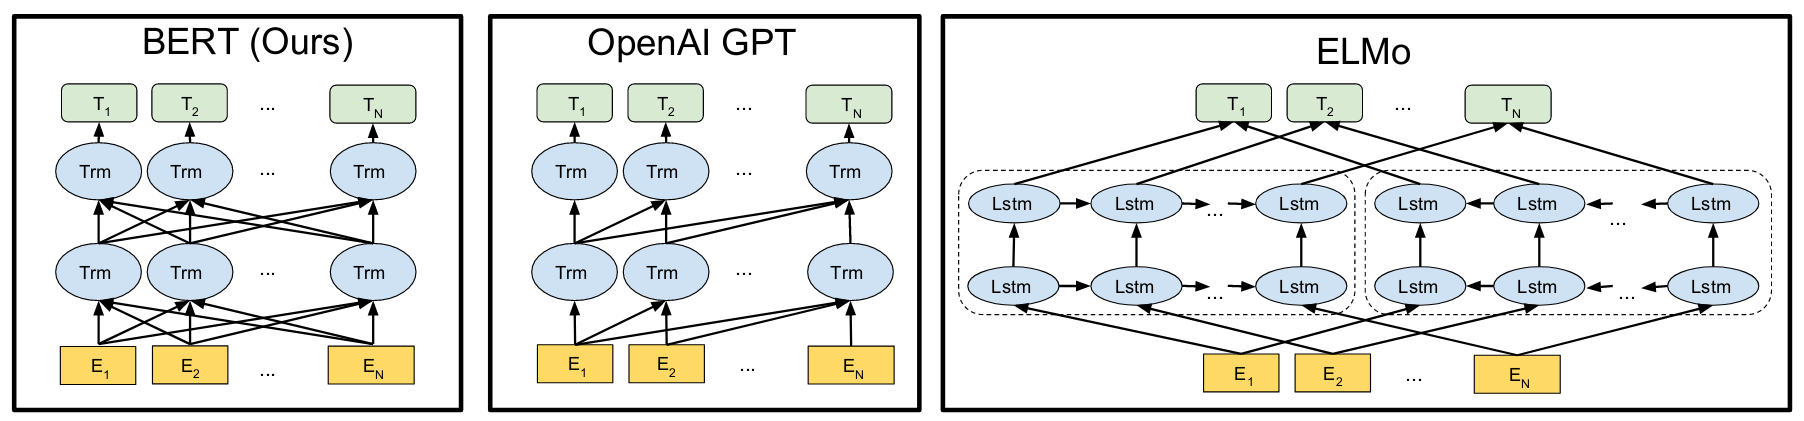
\includegraphics[width=\textwidth]{figures/deeply_bidirectional.png}
    \end{center}
    \caption{
        Comparison of flow of information in the layers of various recent pre-training model architectures~\cite[Figure 1]{devlin2018}.
        Note that ``only BERT representations are jointly conditioned on both left and right context in all layers''~\citep{devlin2018}.
    }
    \label{fig:bert_comparison}
\end{figure}

% available models
Another benefit of BERT is that they provide a wide range of pre-trained models.
The basic models presented in the BERT paper are \bert{base} and \bert{large}.
\bert{base} is ``chosen to have an identical model size as OpenAI GPT for comparison purposes''~\citep{devlin2018}.
\bert{large} obtains higher accuracy on most tasks and has 340 million parameters in total.
Compared to \bert{base} this is an increase from 110 million to 340 million parameters.
The BERT Github repository~\citep{devlin2018github} lists some more models, namely uncased and cased variants for \bert{base} and \bert{large}.
In general uncased models suffice, but for certain tasks (for example, NER) performance can be increased by using a cased model~\citep{devlin2018github}.
Also, they provide \bert{multilingual} and \bert{chinese}.
The multilingual model is trained on the 100 languages having the most Wikipedia pages~\citep{devlin2019multi}.

\subsection{Training}
\label{subsec:training}
% infeasibility of local training
From now on training is used to denote fine-tuning of the model.
Training the general language model on some downstream task is presented as being inexpensive~\citep{devlin2018github}.
Relative to the pre-training it is.
Experiments show that fine-tuning with default hyperparameters will run out of RAM on a 16 GB RAM machine.
Lowering the batch size reduces the memory usage, but running a few training steps still takes at least a few hours.

To train the model on some tasks it is advised to run `a few epochs'~\citep{devlin2018github}.
Based on the example code provided by Google researchers the number of epochs is 3 and the number of training examples is about 1000~\citep{bajaj2018}.
So, it is advised to show the system $3000$ examples.
For our smaller datasets of around 50 examples this means running $3000 / 50 = 60$ epochs.
When measuring the training time in steps it means running $3000 / 16 \approx 188$ steps for a batch size of 16.
Preliminary experiments on the AskUbuntu dataset (having 53 training examples) with a batch size of 32 confirm this estimate, see Figure~\ref{fig:tensorboard}.
The images show that the system does not converge smoothly, and can even have a sudden drop in performance.
One possible explanation for the performance drop is that the model moved into an non-generalizing local minimum.

The results are interesting because it shows that the model is able to learn something even for a dataset with only tens of training examples.
\begin{figure}
    \centering
    \begin{minipage}{0.30\textwidth}
        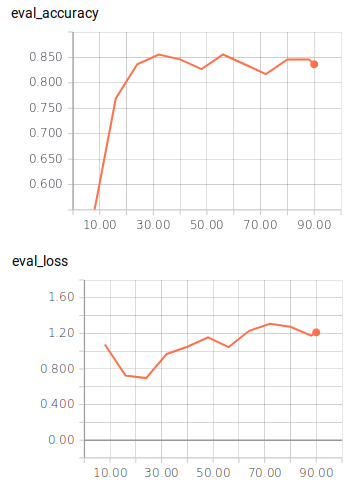
\includegraphics[width=0.9\textwidth]{figures/tensorboard_askubuntu.png}
        \caption*{\bert{base}}
    \end{minipage}
    \hspace*{3mm}
    \begin{minipage}{0.30\textwidth}
        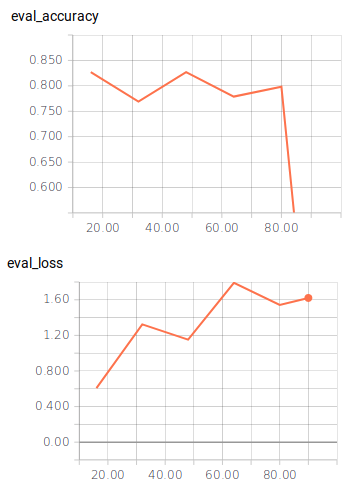
\includegraphics[width=0.9\textwidth]{figures/tensorboard_askubuntu_large.png}
        \caption*{\bert{large}}
    \end{minipage}
    \hspace*{3mm}
    \begin{minipage}{0.30\textwidth}
        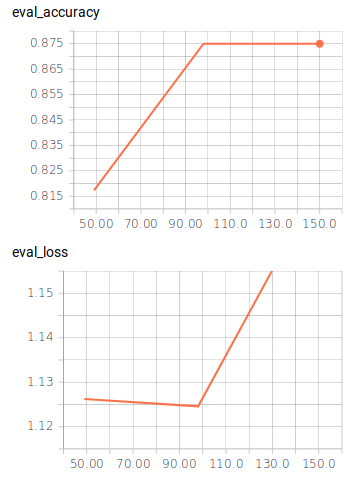
\includegraphics[width=0.9\textwidth]{figures/tensorboard_askubuntu_large_2.png}
        \caption*{\bert{large}, second run}
    \end{minipage}
    \caption{TensorBoard visualisation or `summaries' for fine-tuning pre-trained models on AskUbuntu.
    Here the horizontal axis denotes the number of steps.
    Accuracy and loss for the model trained on the test set is evaluated at fixed steps on the evaluation set.
    The plots show that BERT is in some cases able to converge to a correct local minimum after 100 steps (3200 examples shown to model).
    The scores in these images should not be compared to the scores in Section~\ref{sec:benchmark_results} since the metrics and the data split differ.}
    \label{fig:tensorboard}
\end{figure}
Training the model for 5 steps or 80 examples takes at least a few hours on a modern computer.
Interpolation suggests that training 188 steps will take at least 36 hours.
This is impractical when doing experiments.

% colab intro
According to the paper the benefit of the Transformer models is that they are highly parallelizable.
Training BERT consist mainly of matrix multiplications~\citep{dettmers2018}.
These can be done quickly and efficiently on graphic processing units (GPUs) and tensor processing units (TPUs).
The latter are ASICs created by Google specifically to do machine learning inference~\citep{jouppi2017} and contain 64 GB of RAM~\citep{devlin2018github}.
When using the TensorFlow implementation of BERT GPUs with 16 GB of RAM are required~\citep{devlin2018github}.
GPU optimizations are available in the PyTorch implementation provided by~\citet{wolf2018}, but PyTorch does not support TPUs at the time of writing.
Prices for these GPUs are at least a few thousand euros, which means most users and companies resort to cloud services.
Google Colab~\citet{google2019colab} provides free access to a GPU and TPU instance.
Code which uses Google Colab for BERT is based on an example implementation provided by Google~\citep{bajaj2018}.

% colab usage
Using Colab is a compromise between usability and costs.
The costs are limited to the use of some storage in a Google Cloud Bucket.
Usability is hindered by the usual constraints of online Jupyter Notebook editors, for example no unittests, no autocomplete and poor Git integration.
To overcome these issues most of the code is written and tested locally and pushed to a Github repository called \textsc{improv}, see Appendix~\ref{ch:improv}.
In the Colab the code is then pulled from the repository and main functions are called.
Using Colab has benefits as well.
Hyperparameters and output are visible and can easily be modified in the Notebook, this eases verification.
Reproducibility is possible by opening the Notebook and running all cells.
The first cell will ask to link the Colab to a Google account, make sure this account has access to a Google Cloud Bucket.

% from now on some constraints
The plots in Figure~\ref{fig:tensorboard} are created using the default TensorFlow visualisation tool TensorBoard.
Generating these plots can be done by specifying a model and metrics using the TensorFlow Estimator API.
The plots will not be generated for the rest of the runs for reasons explained in Section~\ref{sec:tpu_and_api}.
For the rest of this document all results are for the \bert{large} model since \bert{base} is only created for a fair comparison with OpenAI GPT~\citep{devlin2018}.

\subsection{Joint training}
\label{subsec:joint_training}
% introduction
One reason why neural networks are obtaining the best results for many fields is because networks are now deep.
Deep networks have more layers and can therefore learn more complex tasks.
One application of this is adding a larger portion of the pipeline to the model.
For example, the code by~\citet{rasa2018config} for the default pipeline for \textsc{rasa-spacy}, as introduced in Section~\ref{subsec:rasa}, contains the following steps.
In these steps a featurizer denotes a system component which transforms text to vector representations~\citep{brutlag2000challenges}.
\begin{enumerate}
    \item Tokenization which splits texts up in tokens.
    \item Regular expression based intent and entity featurizer (for example able to featurize phone numbers),
    \item Intent featurizer based on spaCy~\citep{spacy2019}.
    \item Stanford Named Entity Recognizer based on conditional random fields~\citep{finkel2005incorporating}.
    \item NER synonym detection.
    \item Intent classification based on scikit-learn~\citep{scikit2019}.
\end{enumerate}

For this pipeline the Stanford Named Entity Recognizer and scikit-learn classify separately.
Preferably one would have one model which could learn to do the entire pipeline, also known as an end-to-end model.
End-to-end models have two benefits.
Firstly, an end-to-end model avoids feature engineering and data pre-processing~\citep{ma2016end}.
Secondly, end-to-end models can obtain higher accuracies because (semi-)optimal features are found automatically.

% why it helps
That the combination improves independent models has been shown by~\citet{ma2017jointly} and~\citet{zhang2018joint}.
The results for the former are obtained by using a LSTM network.
The latter introduces an algorithm to combine hidden states from an LSTM.
They show this for the more general problem of sequential labeling and classification.
Intuitively the improvement was to be expected for the following reason.
Suppose we are trying to classify a dataset which contains the sentence:

\begin{center}
    ``I would like to book a ticket to London tomorrow.''
\end{center}

The sentence has intent `BookFlight'.
Training the model could be simplified by providing the sentence classifier with:

\begin{center}
    ``I would like to book a ticket to $<$location$>$ $<$date$>$.''
\end{center}

Now the model does not have to learn to classify sentences while also learning that London is a location and that tomorrow is a date.

% how it should not be done
Note that an end-to-end model is preferred over two separate models.
At the time of writing NER classifiers do not obtain perfect accuracy.
This means that some classifications will be incorrect.
The example from above could instead be converted to:

\begin{center}
    ``I would like to book a $<$date$>$ to $<$location$>$ tomorrow.''
\end{center}

This could make the intent classifier drop in accuracy.
In an ideal end-to-end model incorrect NER classifications would be less of an issue.
The model would learn to ignore the named entity recognition if it would not increase accuracy.

\subsection{BERT joint training}
\label{subsec:bert_joint_training}
% why possible
That joint training BERT is possible can be observed from Figure~\ref{fig:bert_classification}.

\begin{figure}
    \centering
    \begin{minipage}{0.48\textwidth}
        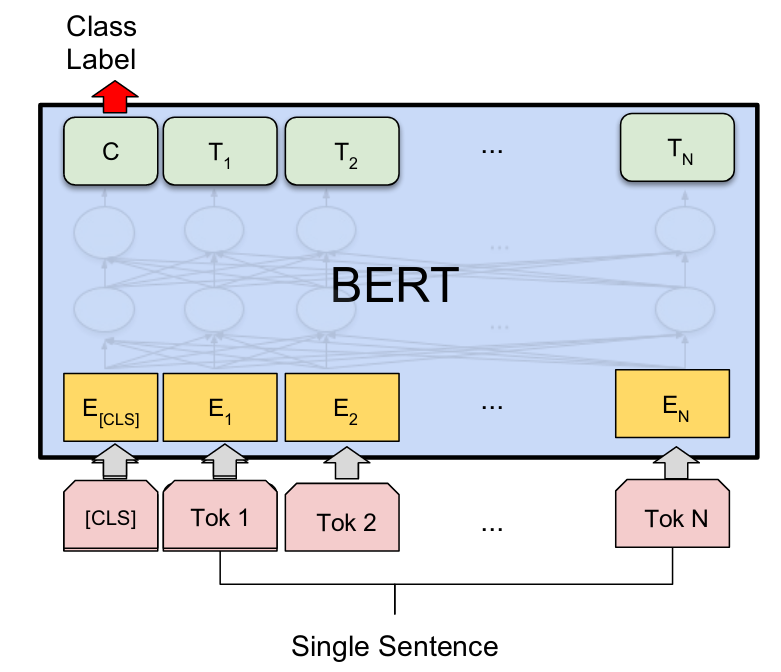
\includegraphics[width=\textwidth]{figures/bert_single_sentence.png}
        \caption*{Single sentence classification}
    \end{minipage}
    \hspace*{3mm}
    \begin{minipage}{0.48\textwidth}
        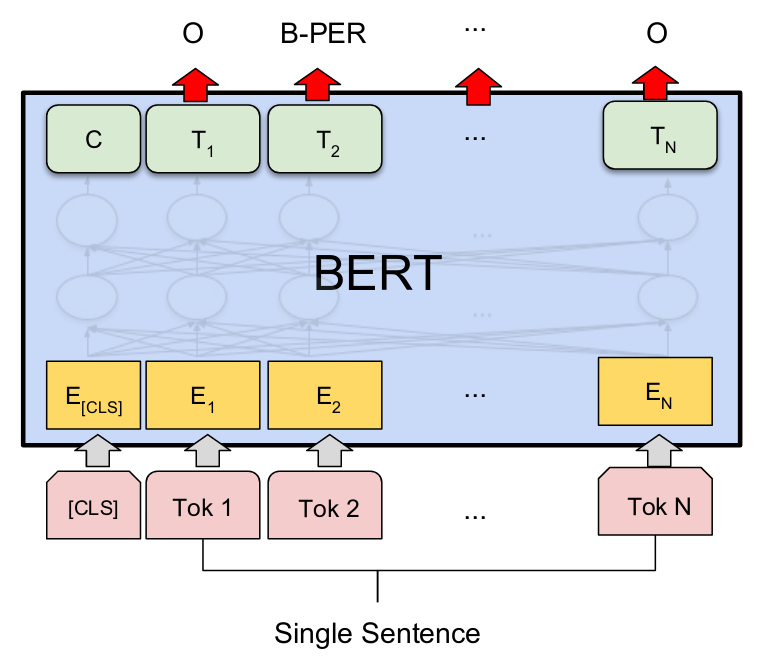
\includegraphics[width=\textwidth]{figures/bert_ner.png}
        \caption*{Single sentence tagging}
    \end{minipage}
    \caption{Two of the four single sentence tasks presented in the BERT publication~\cite[Figure 3]{devlin2018}.}
    \label{fig:bert_classification}
\end{figure}

Let $A = A_1, A_2, \cdots, A_n$ denote the layer which is depicted below $C, T_1, \cdots, T_n$, and let $B = B_1, B_2, \cdots, B_n$ denote the layer below $A$.
Let $s$ denote the number of tokens for some input sentence.
By default the max sequence length for the model is set to 128.
For each sentence the sequence length is padded to this max sequence length.
When predicting a `class label' $C$ will only be based on $A_1$ which is based on $B_1, B_2, \cdots, B_s$.
$A_2, A_3, \cdots, A_n$ are not used.
When predicting entities only $A_2, A_3, \cdots, A_s$ are used.
It seems that a joint model is possible by providing the model with a combination of these two.
Consider the NER as a base model and suppose we add some input to $C$.
Now when predicting $C$ the model is expected to learn to look at input from $A$.
For this it can use entity information from $A_2, A_3, \cdots, A_s$.
To also learn non-trivial patterns in non-entity words in the sentence it can use $A_2, A_3, \cdots, A_n$.
Typically sentences are much shorter than 128 tokens so enough space should be available in $A_2, A_3, \cdots, A_n$.
To allow for more space the max sequence length can be increased, this will increase training and inference time.

% how done
To do this the input for the model has been changed from: \\

\noindent \verb|text: ['how', 'do', 'i', 'disable', 'the', 'spam', 'filter', 'in', 'gmail', '?']|\\
\verb|true: ['O', 'O', 'O', 'O', 'O', 'O', 'O', 'O', 'B-WebService', 'O']|\\

to\\

\noindent \verb|text: ['INTENT', 'how', 'do', 'i', 'disable', 'the', 'spam', 'filter', 'in',|\\
\hspace*{12cm} \verb|'gmail', '?']|\\
\verb|true: ['FilterSpam', 'O', 'O', 'O', 'O', 'O', 'O', 'O', 'O', 'B-WebService', 'O']|\\

where `text' is passed to $C, T_1, \cdots, T_s$ and `true' to $E_{[CLS]}, E_1, \cdots, E_n$ during training.
% In the default BERT model $[CLS]$ is passed to denote that the model is used for classification.
The BERT tokenizer splits words which are not listed in the vocabulary corresponding to a pre-trained model.
INTENT is capitalized to force it to be out-of-vocabulary, it is converted by BERT to [UNK].
The goal of this is to avoid overriding the default interpretation BERT has for `intent' (or any other uncased token we choose).

% loss function
The NER loss function can be applied to the joint training without change.
This is counterintuitive because input examples have one position for the class $C$ and $s$ positions for the entities $T_1, T_2, \cdots, T_s$.
Typically sentences have around 10 tokens after tokenization.
So, the loss is based on around one intent position and ten entities.
This means that the model will learn entity recognition much quicker than intent classification.
For situations where the model is able to learn the entities quickly this is not expected to affect the performance of the intent classification significantly.
% explain more
It is expected that the only significant difference of this change is in the difficulty of the loss function.
% explain morec


\section{Results}
\label{sec:results}

% less text is allowed for this section since it makes sense
Experiments are conducted on the AskUbuntu, Webapplications, Chatbot and SNIPS2017 dataset as introduced in section~\ref{subsec:available_datasets}.
Comparisons are made for a fixed number of steps (or equivalently epochs).
The reason for this is that intermediate results are not easily reported for the BERT model as explained in section~\ref{subsec:training}.
The number of steps to be used for training is basically a guess on what should be enough.
For each dataset various runs for BERT are executed.
During one run only intents are shown to the system and accuracy is measured for intents.
Another run only shows entities and measures intents.
A third run shows the system intents and entities and measures both.
These methods are denoted as separate or joint.
It is expected that the joint training increases accuracy for both intent and entity classifications.
The reason for this is that the model sees more varied data and hence should be able to more easily find a good internal representation of the data.
Results are listed in table~\ref{tab:runs_scores}.

% notes on runs
Note that separate training consists of two runs, and hence ran twice as many epochs.
This seems fair, since intent or entity improvements which require twice as many training steps are not interesting for expensive models such as BERT.
As a baseline Rasa 0.13.8 with the Spacy pipeline is used.
Only intent classification is possible using the benchmark code, so entity scores are missing.
Omitting scores for other systems has been deliberate.
The table is merely meant to support that joint training is feasible.
A final remark is that the scores have been rounded to two decimals.
The reason for this is that results vary between runs and for changes to hyperparameters.
To avoid falsely reporting perfect scores (having accuracy of 1.0), all intent and entity numbers are rounded down.
The number of epochs is calculated by taking number of training steps times training batch size and dividing by number of training examples.
% todo: list number of intents and entities per dataset in table, like discussed in methodology
The training time for each model is around 10 minutes.
Running time differences between runs are small, since most time is spent on training preparations and transferring model checkpoints between TPU and cloud storage.

\begin{table}[htbp]
    \centering
    \begin{tabular}{l l l l l c c}
        \textbf{Dataset}    & \textbf{Steps}  & \textbf{Batch size} & \textbf{Epochs}  & \textbf{Method}   & \textbf{Intent}  & \textbf{Entity}\\
        \hline
        AskUbuntu           & & & & Rasa & 0.83 \\
                            & 250 (twice) & 32 & 151 (twice) &  separate & 0.74 & 0.99\\
                            & 250 & 32 & 151 & joint & 0.98 & 0.79\\
        \hline
        WebApplications     & & & & Rasa & 0.67\\
                            & 250 (twice) & 32 & 267 (twice) & separate & 0.00 & 0.79\\
                            & 250 & 32 & 267 & joint & 0.65 & 0.81\\
                            & 1000 (twice) & 8 & 267 (twice) & separate & 0.72 & 0.79\\
                            & 1000 & 8 & 267 & joint & 0.53 & 0.80\\
        \hline
        Chatbot             & & & & Rasa & 0.98 \\
                            & 250 (twice) & 16 & 40 (twice) & separate & 0.99 & 0.74\\
                            & 250 & 16 & 40 & joint & 0.98 & 0.79\\
        \hline
        Snips2017           & & & & Rasa & 0.99\\
                            & 1500 (twice) & 32 & 22.9 (twice) & separate & 0.03 & 0.83\\
                            & 1500 & 32 & 22.9 & joint & 0.97 & 0.85\\
        \hline
    \end{tabular}
    \caption{Weighted f1 accuracy scores for separate and joint training on four datasets.}
    \label{tab:runs_scores}
\end{table}

The code to reproduce the results the logs (including predictions) can be found at the links provided in table~\ref{tab:runs_urls}.
\begin{table}[htbp]
    \centering
    \begin{tabular}{l l}
        \textbf{Dataset}    & \textbf{Url}\\
        AskUbuntu           & \url{https://github.com/rikhuijzer/improv/tree/master/runs/askubuntu}\\
        WebApps             & \url{https://github.com/rikhuijzer/improv/tree/master/runs/webapplications} \\
        Chatbot             & \url{https://github.com/rikhuijzer/improv/tree/master/runs/chatbot} \\
        Snips2017           & \url{https://github.com/rikhuijzer/improv/tree/master/runs/snips2017} \\
    \end{tabular}
    \caption{Hyperlinks for Rasa and BERT run information.}
    \label{tab:runs_urls}
\end{table}

% result analysis
From the results it can be concluded that joint training is feasible.
The model will not learn anything when training on intents separately for SNIPS2017 and WebApplications.
For WebApplications it has been found that lowering the step size can solve this problem.
This suggests that the gradient descent does not converge because the step size is too big.
A bigger batch size means a more stable error gradient.
It might be that this caused the model to get stuck in a local minimum.
Specifically, the difference with joint training is that the joint training data is much more varied.
Say a typical sentence contains 12 tokens.
Then a joint training batch of size 32 will contain about 3 tokens related to intents and 29 related to entities.
For an intent training batch of size 32 it will contain 32 tokens related to intents.
Hence, the data for the joint training is much more complex.
This seems to indicate that the joint training forces the model to learn a more complex representation.
An alternative explanation could be related to the fact that training data is not shuffled.
The default BERT code hints to shuffle data, but when comparing the Colab log with the training data, the implementation in \textsc{improv} does not.

% closing remarks
An important thing to note about the results is that the datasets are very small.
One would expect that the large BERT model is better suited for datasets which contain more training examples.
Furthermore, the experiments are based on a naive implementation.
Not only the batch size but also other hyperparameters can be tuned for better results.
Training has used a fixed number of steps or epochs.
It might be that more epochs give higher accuracies.
On the other hand it might also be that less epochs correspond to similar accuracies in less training time.
Other interesting hyperparameters are \textit{max\_seq\_length} and \textit{learning\_rate}.
Lowering the former to the expected maximum number of tokens in sentences reduces training and inference time.

Interesting is to observe that jointly training generalizes to sequential labeling and sentence classification.
In other words, any combination of tasks where sentences are classified as well as parts of the sentence and these tasks are correlated.
The tasks are expected to be correlated for any

\iffalse
\section{BERT implementation improvements}
\label{sec:bert_implementation_improvements}
% currently proof of concept, not using I is always preceded by B.
% update loss function
% X and O in NER reducing accuracy of NER
% conditional code to fix I-<entity> statements appearing without B-<entity>
% use multilangual and bert-base etc
% more models
% more datasets
% hyperparameter tuning
\fi


    \clearemptydoublepage

    \chapter{Conclusions}
\label{ch:conclusions}
% intro
Media suggests that difficult natural language processing (NLP) tasks can be solved by using artificial intelligence.
It is interesting to see whether this can be used to automate customer support.
To this end various NLP tasks have been considered.
Eventually it is decided that intent classification is the most interesting task.
Intent classification attempts to classify the intention of some user when he utters some sentence.
For example, ``what is the weather tomorrow?'' could be labeled as `get\_weather'.
A conversational agent (advanced chatbot) could then use this intent to decide how to respond.
% research question one
While reading about this task it was found that various systems claim to have obtained the highest accuracy scores for certain datasets.
This is highly suspicious and gives rise to the following research question and goal.\\

\rqone\\

\rgone\\

The answer for the first research question is that it is possible, but impractical.
Main issue is that to test a service one has to make API calls.
This requires the user of a benchmark tool to have an user account for each service and it forces the tool to update for each changing service.
Another issue is that evaluation of results is done on pre-defined datasets.
This does not guarantee that some system is indeed the best choice for some problem at hand.
It could be that the pre-defined dataset contains more training data, is in another domain or uses another language.
Even when using the benchmarking tool with some use-case specific dataset knowing the best system is not very useful.
Services push new models into production without letting users know, so benchmark results can become invalid at any moment.

%research question two
Next, the tool (and knowledge obtained by creating the tool) is used to work on the following research question and goal.\\

\rqtwo\\

\rgtwo\\

The search for improvement has considered increasing the amount of training data and using new meta-learning algorithms and embeddings.
A recent model called Google BERT~\citep{devlin2018} is expected to be the most likely candidate for increasing accuracy.
The model uses pre-training to learn about language and can be fine-tuned to some specific task.
It is a big model, meaning that fine-tuning takes around 1,5 days on a modern computer and a few minutes on a high-end GPU.
Experiments on intent classification datasets showed non-significant improvements in accuracy.
To improve accuracy further the model has been jointly trained on intent classification and named-entity recognition.
The benefit is that named-entity information can be used to determine the intent and vice versa.
The Google model is a good candidate for jointly training because it uses left and right context in all layers (deep bidirectionality).
BERT has obtained state-of-the-art results in a wide range of tasks including named-entity recognition.
This implies that jointly training BERT should obtain state-of-the-art results on the natural language understanding task.
Specifically, on tasks where data consists of intents and named-entities which is typical for conversational agents.
Basic experiments are conducted in which training BERT separately is compared to training it jointly.
The experiments show that jointly training is possible and in some cases obtains higher accuracies than separate training.
It is expected that the results can be improved by taking a second look at the implementation and improving it.
One issue for the current implementation is that the implementation does not shuffle the training data.

\iffalse
% conclusions
In general the NLP field is in an interesting state.
Technology companies have a lot of incentive to push the field forward.
Leaps in the last few years have come from those companies.
For example, FastText by Facebook and transformer models by Google.
A second observation is that state-of-the-art scores are increased every few months.
This results in papers which are quickly pushed to arXiv and cited before any scholarly peer review.
Papers report accuracy high scores with ``few mentions of average cases and variability or worst-cases''~\citep{otter2018survey}.
\fi
% this cautionary conclusion is mainly from first part of thesis
% check number of arxiv citations in review paper, ~64 of 190 citations are arXiv

% todo: mention that the approach generalizes to task


    \clearemptydoublepage

    %Choose a good bibliography style, plain would do often, but these might be nice too
    %\bibliographystyle{these}
    \bibliographystyle{plainnat}
    \bibliography{references}

    \clearemptydoublepage

    \appendix
    \addcontentsline{toc}{chapter}{Appendix}

    \chapter{\textsc{bench}}
\label{ch:bench}

% intro
The benchmarking tool is called \textsc{bench} and located on Github (\url{https://github.com/rikhuijzer/bench}).
Its goal is to be a reproducible benchmarking tool for intent classification and named-entity recognition.
Reproducible means that other people can run the code for their own use, or to reproduce results presented in this report.
The code is written in Python, since it is the default choice for machine learning.
Python is conceived as a object oriented language.
Over time it has included more and more functional programming ideas.
The code in this project will aim to be adhering to functional programming.
Reasons are pedagogic value, improved modularity, expressiveness, ease of testing, and brevity.
Some general notes on functional programming in Python are listed in Appendix~\ref{ch:fp}.

% final code remarks on fp and imports
The functional programming constraints for the project are that we do not define any new classes.
Specifically, we do not use the class keyword.
Exceptions being NamedTuples and Enums.
Both do provide functional APIs, but these are not fully supported by the autocomplete in PyCharm.
The code prefers returning iterators over collections, the reason for this is explained in Appendix~\ref{ch:demonstration}.
A final remark is about the imports.
When importing an attempt is made to explicitly import using `from $<$module$>$ import $<$class$>$`.
When more implicit imports are used `import $<$module$>$` this is can have multiple causes.
It is either caused by the appearance of circular imports, by the fact that some names are too common or to avoid reader confusion.
An example for the latter are the types defined in \textsc{src.typ}.
The names are quite generic and could cause name clashing or confusion when imported explicitly.

\section{Usage}
\label{sec:usage}
% set-up
Installation is similar to other Python projects.
Pull the code and in a terminal set the current working directory to the project folder.
Install the required pip packages by running the following command.
\begin{verbatim}
    pip install -r requirements.txt
\end{verbatim}
If one wants to check accuracy for an open-source system then run the following command.
\begin{verbatim}
    docker-compose up
\end{verbatim}
\textsc{docker-compose} will read `docker-compose.yml' and use that information to spin up various Docker containers.
All dockers listed in the file are available from Docker Hub.
This avoids having to build Dockers manually.
DeepPavlov has been removed from the configuration file, since it was found to be unstable, see Section~\ref{subsec:deeppavlov}.

% final parameters and run
After the set-up the program can be executed by running `bench.py'.
To change on which system the benchmarking occurs, replace the first parameter in the \textsc{get\_system\_corpus} call.
The prefix is used to determine which system is being tested.
Possible prefix options are `mock', `rasa', `deeppavlov', `lex' and `dialogflow'.
Rasa and DeepPavlov will use the complete string to find a matching port from `docker-compose.yml'.
So, based on the Docker configuration one can also specify `rasa-tensorflow', `rasa-spacy' or `rasa-mitie'.
The corpus (dataset) to run the bench on is specified by an enumerable, see \textsc{src.typ.Corpus} for possible options.
When running the script in a modern IDE autocomplete will suggest the possible corpora.
Slightly more convenient would be to have the script take input arguments using \textsc{sys.argv}.
After setting the two parameters the script can be executed and will display all predictions as well as micro, macro and weighted f1 scores.
The predictions and f1 scores will also be written to files, see the `results' folder.

\section{Overview}
\label{sec:overview}
A high-level code overview will be presented.
Since the code does not contain classes, the overview is simply a tree-like structure.
This is analogous with a book, where subsections are contained in sections and sections are contained in chapters.
In the code small functions are called by larger functions and these larger functions are called by even larger functions.
For an overview this idea can be generalized to modules.
An overview for the modules of \textsc{bench} is roughly as follows.
The `.py' suffix is omitted for all elements in the tree.
Tests are also omitted.

\begin{itemize}
    \item \textsc{bench}
    \begin{itemize}
        \item \textsc{src.utils}
        \item \textsc{src.typ}
        \item \textsc{src.dataset}
        \begin{itemize}
            \item \textsc{src.datasets.corpora}
            \item \textsc{src.datasets.snips}
        \end{itemize}
        \item \textsc{src.system}
        \begin{itemize}
            \item \textsc{src.systems.amazon\_lex}
            \item \textsc{src.systems.deeppavlov}
            \item \textsc{src.systems.dialogflow}
            \item \textsc{src.systems.mock}
            \item \textsc{src.systems.rasa}
            \item \textsc{src.systems.watson}
        \end{itemize}
        \item \textsc{src.evaluate}
        \begin{itemize}
            \item \textsc{src.results}
        \end{itemize}
    \end{itemize}
\end{itemize}

Some generic functions are listed in \textsc{src.utils} and used through the entire project.
The project makes use of type hints as introduced in Python 3 (and via comments in Python 2.7).
Also, the project does not use classes and therefore tends to pass more data through functions.
To define containers for these data NamedTuples are used.
A more in-depth explanation of why these are needed can be found in Section~\ref{sec:named_tuple}.
All NamedTuples or `types' are defined in \textsc{src.typ}.
The module also contains enumerable's or `Enums'.
These are used in cases where function behaviour depends on some parameter from a fixed set of options.
Alternatively one could use strings for these cases depending on user-preference.

The real work of the project is done by \textsc{src.dataset}, \textsc{src.system} and \textsc{src.evaluate}.
`Dataset' takes input files and converts them to an internal representation as defined by \textsc{src.typ}.
Input files here denote the original dataset files as created by the dataset publishers.
For the internal representation a Rasa Message is used, specifically \textsc{rasa\_nlu.training\_data.message.Message}.
The benefit of this is that it avoids defining the same structure and that it can be used in combination with Rasa code.
For example, \textsc{src.dataset.convert\_message\_to\_annotated\_str} uses Rasa code to print the internal data representation as a sentence in Markdown format (Section~\ref{subsec:format}).
Next, the data reaches \textsc{src.system}.
Here it is passed to the system under consideration, either in training or prediction mode.
For the predictions this is done by finding out which function can convert \textsc{src.typ.Query} to \textsc{src.typ.Response}.
When, for example, Rasa is under consideration the function \textsc{src.systems.rasa.get\_response} is called.
DeepPavlov would be handled by \textsc{src.systems.deeppavlov.get\_response}.
PyCharm is known to have the best type inference for Python.
The IDE is not yet able to infer function type for a function mapping, even when all functions have the same input and output type.
A workaround is to manually define the type of the function returned by the mapping as \verb|func: Callable[[tp.Query], tp.Response] =| $\cdots$.
\textsc{src.evaluate} takes all responses \textsc{tp.Response} evaluates the performance of the system under consideration.
Printing f1 score is a matter of three functions and about a dozen lines of code.
At one point more advanced logging has been included which is responsible for the other 12 functions and 110 lines of code.


    \chapter{Notes on functional programming in Python}
\label{ch:fp}

Python is not a pure functional language.
However more and more constructs of functional programming are being added to the language each year.
This appendix will explain some functional ideas used in the code, as presented by~\citet{lott2015}.
Higher-order functions take or return functions, this is used to replace the factory design pattern as explained in Section~\ref{sec:mapping_to_functions}.
Keeping track of state without a class results in function signatures to contain many parameters, these can be handled by using NamedTuples, see Section~\ref{sec:named_tuple}.
Another benefit of classes is that data can be stored, used for example in caching.
A convenient solution for caching is described in Section~\ref{sec:function_caching}.
Collections of data are typically transformed via loops.
Here each loop will transform the entire collection and move to the next transformation.
Lazy evaluation, as described in Section~\ref{sec:lazy_evaluation}, uses a more efficient way.

\section{Mapping to functions}
\label{sec:mapping_to_functions}
In code we often have a function which calls other functions depending on some conditionals.
For example in `system.py` the factory design pattern is replaced by a more functional design.
In this design `system.py` behaves like a super and delegates the work based on what system
we currently interested in.
We give an example for two systems.
The delegation could be done via conditional statements.

\begin{verbatim}
    if 'mock' in system.name:
      response = src.systems.mock.get_response(tp.Query(system, message.text))
    elif 'rasa' in system.name:
      response = src.systems.rasa.get_response(tp.Query(system, message.text))
    elif ...
\end{verbatim}

This introduces a lot of code duplication.
Therefore a dict is created.
\begin{verbatim}
    get_intent_systems = {
      'mock': src.systems.mock.get_response,
      'rasa': src.systems.rasa.get_response,
      ...
    }
\end{verbatim}
Now we can just get the correct function from the dict and call it.
\begin{verbatim}
    func: Callable[[tp.Query], tp.Response] =
      get_substring_match(get_intent_systems, system.name)
    query = tp.Query(system, message.text)
    response = func(query)
\end{verbatim}

Note that \textsc{get\_substring\_match()} implements the substring matching used in the conditional code (\textsc{if 'mock' in system.name:}).
Since the code can return any of the functions contained in the mapping they should all have the same signature and output.
The used IDE (PyCharm 2018.2.4) is not able to check this.
Therefore, functions from the mapping \textsc{func} get a type hint.
This allows the IDE to check types again and it allows developers to see what signature should be used for all the functions in the mapping.

\section{NamedTuple}
\label{sec:named_tuple}
Pure functions by definition cannot rely on information stored somewhere in the system.
We provide one example from the code where this created a problem and how this can be solved using NamedTuples.

The benchmarking tools communicates with a system called Rasa.
Rasa starts in a default, untrained, state.
To measure its performance we train Rasa and then send many sentences to the system.
In general one prefers to functions should be as generic as possible.
It makes sense to have one function which takes some sentence, sends it to Rasa to be classified and returns all information from the response.
To avoid re-training Rasa for each system we have to remember whether Rasa is already trained.
Passing a flag 'retrain' to the system is insufficient, since the function does not know where Rasa should train on.
To make it all work we need the following parameters:
\begin{itemize}
    \item \textsc{sentence}: The sentence text.
    \item \textsc{sentence\_corpus}: The corpus the sentence is taken from.
    \item \textsc{system\_name}: Used to call the function which can train the specific system we are interested in.
    \item \textsc{system\_knowledge}: Used in combination with \textsc{sentence\_corpus} to determine whether we need to re-train.
    \item \textsc{system\_data}: In specific cases even more information is needed.
\end{itemize}
re-training the system to check whether its outputs differ.

When this function has decided to train the system the system\_knowledge changes.
% todo: what should be on next line
So as output we need to return ``

Since Python 3.5 a NamedTuple with type hints is available.

To allow for better type checking and reduce the number of function parameters use is made of \textsc{typing.NamedTuples}.

% todo: Explain how NamedTuples help type checking on Factory Design pattern replacement.

\section{Function caching}
\label{sec:function_caching}
Functions can be cached using \textsc{functools.lru\_cache}.
This is mainly used for reducing the number of filesystem operations.
A typical example is as follows.
Suppose we write some text to a file iteratively by calling \textsc{write} multiple times.
Since we try to avoid storing a state \textsc{write} does not know whether the file already exists.
To solve we can do two things.
The first option is passing parameters telling the function whether the file already exists.
This is cumbersome, since this state needs to be passed through all the functions to the function which is calling the loop over \textsc{write}.
This can be done directly by calling \textsc{write} or indirectly by calling some other function.
The second option is defining a function to create a file if it does not yet exists \textsc{create\_file}.
We call this function every time \textsc{write} is called.
This does mean that the filesystem is accessed to check the folder each time \textsc{write} is called.
To avoid all those filesystem operations \textsc{create\_file} can be decorated using \textsc{functools.lru\_cache}.
Now on all but the first calls to \textsc{create\_file} just query memory.

% caveats
There is one caveat with this using function caching.
Make sure to not try to mimic state.
In other words the program should not change behaviour if the cache is removed.
Reason for this is that any state introduced via the cache is similar to creating functions with side-effects but without all the constructs from object-oriented programming.

\section{Lazy evaluation}
\label{sec:lazy_evaluation}
By default Python is not interested in performance and advises to use a list for every collection.
However, lists are mutable and therefore not suitable for hashing.
Since hashing is not possible any function taking lists as input is not suitable for function caching.

Also, in many cases the list might not be the final structure we need.
Consider the following use cases where the output of type list is used:
\begin{itemize}
    \item Only unique values are required, so the list is casted to a set.
    \item Only whether some value satisfies P is required.
    \item The x first elements are required.
    \item Only the values satisfying x are required.
    \item Only an output which is transformed is required.
\end{itemize}

Considering all these use cases it makes more sense to return an iterator by default instead of a collection.
One practical example for the bench project which supports this notion is using an iterator on classification requests.

Suppose we want to measure the performance of some cloud service.
Suppose we wrote some code which takes a sentence from some corpus and performs the following operations on this sentence:
\begin{enumerate}
    \item Send the sentence to some cloud service.
    \item Transforms the response to the pieces of information we need.
    \item Store this information.
\end{enumerate}
Suppose one of the last two operations contains a mistake causing the program to crash.
When not using an iterator all sentences will have been sent to the cloud service after the first operation.
Since the post-processing did not succeed we did not obtain results and need to redo this operation.
In effect the programming error caused us to waste about as many API calls as there are sentences in the corpus we are testing.
This is a problem since the API calls cost money and take time to execute.

To solve this use lazy evaluation.
For example, functions supporting lazy evaluation in Python are \textsc{map}, \textsc{filter}, \textsc{reduce} and \textsc{any}.
Another benefit for using iterators is that it improves modularity and, once used to the paradigm, readability.
Take the following typical Python code.

\begin{verbatim}
    my_list = []
    for item in some_iterable:
      updated_item = g(f(item))
      my_list.append(updated_item)
\end{verbatim}

In this code some iterable is read and the transformation \textsc{f} and \textsc{g} are applied to each item in the iterable.
The same code can be rewritten to use \textsc{map} as follows.

\begin{verbatim}
    def transform(item: SomeType) -> OtherType:
      return g(f(item))

    my_iterable = map(transform, some_iterable)
\end{verbatim}


    \chapter{Lazy evaluation demonstration}
\label{ch:demonstration}

This appendix demonstrates the effect of using iterators instead of regular collections.
The code demonstrates this by processing some fictional raw materials to a chair.
The first is function called \textsc{ford} is similar to a Ford factory around 1915.
Here each part of the assembly line just keeps producing items as long as there is input coming in.
After a while the other parts of the assembly line start processing the items and discover a fault in the items.
One problem of this way of working is that the factory now has a pile of incorrect items in their stock.

The second function called \textsc{toyota} is similar to a Toyota factory after 1960.
Here just-in-time (JIT) manufacturing is used as developed by Toyota~\citep{ohno1988toyota}.
Each item is processed only when the next step in the process makes a request for this item.

\section{Benefits}
\label{sec:benefits}
Using JIT makes sense in computer programs for the following reasons.
It saves memory.
In each step in the process we only store one intermediate result instead of all intermediate results.

It can detect bugs earlier.
Suppose you got a combination of processing steps, lets call them \textsc{f} and \textsc{g} and you apply them to 100 items.
In \textsc{f} we send some object to a system and get a response.
In \textsc{h} we store the response of this API call.
Suppose there is a bug in \textsc{h}, lets say the file name is incorrect.
Suppose this is not covered in the tests and we decide to run our program to get all the results we want.
Using an approach similar to \textsc{ford} the program crashes after doing 100 executions of \textsc{f} and \textsc{g}.
This means that the program executed 100 API calls.
Using \textsc{toyota} the program crashes after just one API call.
Here \textsc{ford} has in essence wasted 99 API calls.

It does not make assumptions for the caller.
Suppose some function \textsc{k} returns an iterable and is called by \textsc{l}.
The function \textsc{l} can now decide how it wants to use the iterable.
For example it can be casted to unique values via \textsc{set} or it can partly be evaluated by using \textsc{any}.

\section{Code}
\label{sec:code}
\begin{verbatim}
from typing import List, NamedTuple
""" See README.md """

Wood = NamedTuple('Wood', [('id', int)])
Chair = NamedTuple('Chair', [('id', int)])


materials = [Wood(0), Wood(1), Wood(2)]


def ford():
    """ Processing all the items at once and going to the next step. """
    def remove_faulty(items: List[Wood]) -> List[Wood]:
        out = []
        for material in items:
            print('inspecting {}'.format(material))
            if material.id != 1:
                out.append(material)
        return out

    def process(items: List[Wood]) -> List[Chair]:
        out = []
        for material in items:
            print('processing {}'.format(material))
            out.append(Chair(material.id))
        return out

    filtered = remove_faulty(materials)
    processed = process(filtered)
    print('Result of ford(): {}'.format(processed))


def toyota():
    """ Processing all the items one by one. """
    def is_not_faulty(material: Wood) -> bool:
        print('inspecting {}'.format(material))
        return material.id != 1

    def process(material: Wood) -> Chair:
        print('processing {}'.format(material))
        return Chair(material.id)

    filtered = filter(is_not_faulty, materials)
    processed = list(map(process, filtered))
    print('Result of toyota(): {}'.format(processed))


if __name__ == '__main__':
    ford()
    print()
    toyota()
\end{verbatim}

\section{Output}
\label{sec:output}
The output for the program is as follows.

\begin{verbatim}
inspecting Wood(id=0)
inspecting Wood(id=1)
inspecting Wood(id=2)
processing Wood(id=0)
processing Wood(id=2)
Result of ford(): [Chair(id=0), Chair(id=2)]

inspecting Wood(id=0)
processing Wood(id=0)
inspecting Wood(id=1)
inspecting Wood(id=2)
processing Wood(id=2)
Result of toyota(): [Chair(id=0), Chair(id=2)]
\end{verbatim}

This demonstrates that iterator elements are only executed when called.


    \chapter{Intent f1 score calculations}
\label{ch:intent_f1_score_calculations}

The f1 score calculation by~\citep{braun2017} uses micro averaging.
For two reasons this appendix focuses these calculations on intent only.
The first reason is that these results are compared against benchmarks from the \textsc{bench} project in Section~\ref{sec:benchmark_results}.
Secondly, micro averages could be skewed when the number of intents and entities differ, as described in Section~\ref{subsec:methodology}.
It is interesting to compare the differences.
This appendix lists calculations for Rasa in Section~\ref{sec:recalculations_rasa}, Watson Conversation in Section~\ref{sec:recalculations_watson} and Microsoft LUIS in Section~\ref{sec:recalculations_luis}.

\section{Rasa}
\label{sec:recalculations_rasa}
\vspace*{1cm}

\begin{center}
    \begin{tabular}{l l l l l l l l}
        \textbf{Corpus} & \textbf{Intent} & \textbf{True +} & \textbf{False -} & \textbf{False +} & \textbf{Prec-} & \textbf{Recall} & \textbf{F1}\\
        & & & & & \textbf{ision} & & \textbf{score} \\
        \hline
        \multirow{3}{*}{Chatbot} & DepartureTime & 34 & 1 & 1 & 0.971 & &  \\
        & FindConnection & 70 & 1 & 1 & 0.986 & 0.986 & 0.986 \\
        & $\Sigma$ & 104 & 2 & 2 & 0.981 & 0.981 & \textbf{0.981} \\
        \hline
        \multirow{9}{*}{WebApps} & ChangePassword & 4 & 2 & 0 & 1 & 0.667 & 0.8 \\
        & DeleteAccount & 9 & 1 & 5 & 0.643 & 0.9 & 0.75 \\
        & DownloadVideo & 0 & 0 & 1 & 0 & &  \\
        & ExportData & 0 & 3 & 0 & & 0 &  \\
        & FilterSpam & 13 & 1 & 0 & 1 & 0.929 & 0.963 \\
        & FindAlternative & 15 & 1 & 8 & 0.652 & 0.938 & 0.769 \\
        & None & 0 & 4 & 1 & 0 & 0 &  \\
        & SyncAccounts & 3 & 3 & 0 & 1 & 0.5 & 0.667 \\
        & $\Sigma$ & 44 & 15 & 15 & 0.746 & 0.746 & \textbf{0.746} \\
        \hline
        \multirow{6}{*}{AskUbuntu} \hspace*{-3mm} & MakeUpdate & 34 & 3 & 2 & 0.944 & 0.919 & 0.931 \\
        & SetupPrinter & 13 & 0 & 2 & 0.867 & 1 & 0.929 \\
        & ShutdownComputer \hspace*{-3mm} & 14 & 0 & 6 & 0.7 & 1 & 0.824 \\
        & SRecommendation & 33 & 7 & 4 & 0.892 & 0.825 & 0.857\\
        & None & 0 & 5 & 1 & 0 & 0 \\
        & $\Sigma$ & 94 & 15 & 15 & 0.862 & 0.862 & \textbf{0.862}\\
        \hline
    \end{tabular}
\end{center}

\section{Watson Conversation}
\label{sec:recalculations_watson}
\vspace*{1cm}

\begin{center}
    \begin{tabular}{l l l l l l l l}
        \textbf{Corpus} & \textbf{Intent} & \textbf{True +} & \textbf{False -} & \textbf{False +} & \textbf{Prec-} & \textbf{Recall} & \textbf{F1}\\
        & & & & & \textbf{ision} & & \textbf{score} \\
        \hline
        \multirow{3}{*}{Chatbot} & DepartureTime & 33 & 2 & 1 & 0.971 & 0.943 & 0.957 \\
        & FindConnection & 70 & 1 & 2 & 0.972 & 0.986 & 0.979 \\
        & $\Sigma$ & 103 & 3 & 3 & 0.972 & 0.972 & \textbf{0.972} \\
        \hline
        \multirow{9}{*}{WebApps} & ChangePassword & 5 & 1 & 0 & 1 & 0.833 & 0.909 \\
        & DeleteAccount & 9 & 1 & 3 & 0.75 & 0.9 & 0.818 \\
        & DownloadVideo & 0 & 0 & 1 & 0 & &  \\
        & ExportData & 2 & 1 & 2 & 0.5 & 0.667 & 0.572 \\
        & FilterSpam & 13 & 1 & 2 & 0.867 & 0.929 & 0.897 \\
        & FindAlternative & 15 & 1 & 1 & 0.938 & 0.938 & 0.938 \\
        & None & 0 & 4 & 1 & 0 & 0 &  \\
        & SyncAccounts & 5 & 1 & 0 & 1 & 0.833 & 0.909 \\
        & $\Sigma$ & 49 & 10 & 10 & 0.831 & 0.831 & \textbf{0.831} \\
        \hline
        \multirow{6}{*}{AskUbuntu} & MakeUpdate & 37 & 0 & 4 & 0.902 & 1 & 0.948 \\
        & SetupPrinter & 13 & 0 & 1 & 0.929 & 1 & 0.963 \\
        & ShutdownComputer & 14 & 0 & 1 & 0.929 & 1 & 0.963 \\
        & SRecommendation & 35 & 5 & 3 & 0.921 & 0.875 & 0.897\\
        & None & 1 & 4 & 1 & 0.5 & 0.2 & 0.286 \\
        & $\Sigma$ & 100 & 9 & 9 & 0.917 & 0.917 & \textbf{0.917}\\
        \hline
    \end{tabular}
\end{center}

\section{Microsoft LUIS}
\label{sec:recalculations_luis}
\vspace*{1cm}

\begin{center}
    \begin{tabular}{l l l l l l l l}
        \textbf{Corpus} & \textbf{Intent} & \textbf{True +} & \textbf{False -} & \textbf{False +} & \textbf{Prec-} & \textbf{Recall} & \textbf{F1}\\
        & & & & & \textbf{ision} & & \textbf{score} \\
        \hline
        \multirow{3}{*}{Chatbot} & DepartureTime & 34 & 1 & 1 & 0.971 & 0.971 & 0.971 \\
        & FindConnection & 70 & 1 & 1 & 0.986 & 0.986 & 0.986 \\
        & $\Sigma$ & 104 & 2 & 2 & 0.981 & 0.981 & \textbf{0.981} \\
        \hline
        \multirow{9}{*}{WebApps} & ChangePassword & 3 & 3 & 0 & 1 & 0.5 & 0.667 \\
        & DeleteAccount & 8 & 2 & 0 & 1 & 0.8 & 0.889 \\
        & DownloadVideo & 0 & 0 & 0 & & &  \\
        & ExportData & 3 & 0 & 1 & 0.75 & 1 & 0.857 \\
        & FilterSpam & 12 & 2 & 0 & 1 & 0.857 & 0.923 \\
        & FindAlternative & 14 & 2 & 2 & 0.875 & 0.875 & 0.875 \\
        & None & 3 & 1 & 8 & 0.273 & 0.75 & 0.4  \\
        & SyncAccounts & 5 & 1 & 0 & 1 & 0.833 & 0.909 \\
        & $\Sigma$ & 48 & 11 & 11 & 0.814 & 0.814 & \textbf{0.814} \\
        \hline
        \multirow{6}{*}{AskUbuntu} & MakeUpdate & 36 & 1 & 4 & 0.9 & 0.973 & 0.935 \\
        & SetupPrinter & 12 & 1 & 2 & 0.857 & 0.923 & 0.935 \\
        & ShutdownComputer & 14 & 0 & 0 & 1 & 1 & 1 \\
        & SRecommendation & 36 & 4 & 5 & 0.878 & 0.9 & 0.889\\
        & None & 0 & 5 & 0 & & 0 & \\
        & $\Sigma$ & 98 & 11 & 11 & 0.899 & 0.899 & \textbf{0.899}\\
        \hline
    \end{tabular}
\end{center}


    \iffalse
    \chapter{\textsc{improv}}
\label{ch:improv}
% intro
The project aimed to improve accuracy is called \textsc{improv} and available on Github (\url{https://github.com/rikhuijzer/improv}).
One warning for people interested in reading or using this code is that it is in need of refactoring.
The code is cloned from the Google BERT code, built on the Google TensorFlow library, as provided by the researchers~\citep{devlin2018github}.

% pytorch
Alternatively, code is available for the PyTorch library~\citep{wolf2018github}.
The PyTorch implementation is under active development unlike the TensorFlow implementation and includes more functionality.
Features include Multi-GPU, distributed and 16-bits training.
These allow the model to be trained more easily on GPUs by reducing and distributing the memory used by the model.
BERT contains various models including \bert{base} and \bert{large}.
Since Google Colab does not provide a multi-GPU set-up, we need to use a TPU.
This is not yet supported by PyTorch~\citep{wolf2018github}.

\section{Usage}
\label{sec:improv_usage}
The \textsc{improv} code can partially be executed on a local system.
However, training the model requires at least one enterprise grade GPU.
This is discussed in Section~\ref{subsec:training}.
GPUs and TPUs are provided for free by Google Colab~\citep{google2019colab}.
Using this code means importing one of IPython Notebooks from the \textsc{improv} repository in Colab.
Hyperparameters can be set in the Notebook after which the code can be executed.
The Notebook require a Google Account combined with a paid Google Cloud Bucket.
The Bucket is used to store the trained checkpoints created by training the model.
Newer runs listed in the `runs' folder in the Github repository depend on \textsc{improv}, \textsc{nlu\_datasets} and \textsc{rasa\_nlu}.
The dependencies list the used version in the Notebook.
When errors occur make sure that the correct versions are cloned or installed.

\iffalse
\section{Overview}
\label{sec:improv_overview}
Since the code is in need of refactoring this section will only describe the most important parts of the project.

\fi

% todo: describe estimator API and why it does not work

    \chapter{\textsc{nlu\_datasets}}
\label{ch:nlu_datasets}


    \fi
\end{document}
